\documentclass{SGGW-thesis}
\usepackage{xcolor,amsfonts}
\NewCommandCopy{\amshbar}{\hbar}

\INZYNIERSKAtrue
\WZIMtrue

\title{Wykorzystanie technologii webowych i języka Python do stworzenia aplikacji edukacyjnej z mechaniki kwantowej}
\Etitle{Utilizing web technologies and Python language to create quantum physics educational application}

\author{Adrian Rostek}
\album{205860}
\thesis{Praca dyplomowa na kierunku:}
\course{Informatyka}
\promotor{dr. Andrzeja Zembrzuskiego}
\pworkplace{Instytut Informatyki Technicznej\\Katedra Systemów Informatycznych}

\usepackage{hyperref}
\usepackage{amsmath}
\usepackage{float}
\usepackage{graphicx}
\usepackage{subcaption}

\begin{document}
\maketitle
\statementpage
\abstractpage
{Wykorzystanie technologii webowych i języka Python do stworzenia aplikacji edukacyjnej z mechaniki kwantowej}
{Celem niniejszej pracy było stworzenie aplikacji edukacyjnej do nauki zagadnień mechaniki kwantowej. Zagadnienia podzielone zostały na sześć rozdziałów, w których za pomocą interaktywnych wizualizacji, użytkownik może nauczyć się o istocie i zachowaniu funkcji falowej. Aplikacja przy użyciu frameworka Tauri, stworzona została z wykorzystaniem technologii webowych - języków HTML, CSS i TypeScript, ale korzysta również z języka Python do wykonywania obliczeń fizycznych.}
{Edukacja, Fizyka kwantowa, Funkcja falowa, Wizualizacja}
{Utilizing web technologies and Python language to create quantum physics educational application}
{The goal of this thesis was to create and educational app for learning quantum mechanics. Material was divided into six chapters in which a user can learn about importance and behaviour of wave function via interactive visualizations. Application was created with the use of Tauri framework and web technologies - HTML, CSS and TypeScript languages but it also uses Python langauge for physics calculations.}
{Education, Quantum physics, Wave function, Visualization}


{
  % Spis treści może być złożony z pojedynczą interlinią, np. jeśli jedna linia wychodzi na następną stronę.
  % W przeciwnym razie spis treści wstawić bez powyższego rozkazu i klamry.
  \doublespacing
  \tableofcontents
}

\startchapterfromoddpage % niezależnie od długości spisu treści pierwszy rozdział zacznie się na nieparzystej stronie

\chapter{Wstęp}
Stworzenie mechaniki kwantowej okazało się niezwykle istotne dla dzisiejszej cywilizacji. Zawdzięczamy jej m.in. tranzystory oraz reaktory jądrowe, bez których ciężko wyobrazić sobie dzisiejszą energetykę \cite{nuclear-stats}. Mimo to jest to bardzo nieintuicyjny i przez większość ludzi niezrozumiały dział fizyki \cite{fiz atom}. Na temat ten napisane zostały liczne publikacje \cite{fiz atom} \cite{mechanika kwant} \cite{fiz kwant}, jednak profesjonalny język i matematyka wyższa mogą sprawić dużo trudności w zrozumieniu nawet podstawowych konceptów tej teorii.

	\section{Cel i motywacja pracy}
	Celem pracy jest stworzenie aplikacji, która ma ułatwić naukę zagadnień z zakresu mechaniki kwantowej. Zagadnienia przedstawiane są w interaktywny sposób celem podtrzymania uwagi i zainteresowania tym nietrywialnym tematem. Osiągnięte to zostało poprzez wykorzystanie szeregu prezentacji wizualnych, na których efekt końcowy bezpośredni wpływ ma użytkownik. Zastosowany został również samouczek, który te efekty odpowiednio tłumaczy.
	
	Osobiście temat mechaniki kwantowej uważam za niezwykle ciekawy, więc napisanie tej pracy motywowane jest chęcią poszerzenia swojej wiedzy w tym obszarze, jak i zastosowaniu nabytej wiedzy informatycznej w stworzeniu praktycznego narzędzia. Za interesujące również uważam symulację funkcji falowej w przeciwieństwie do przypatrywania się statycznym jej wykresom na papierze czy w plikach pdf. Aplikacja kierowana jest do osób chcących nauczyć się wstępnych zagadnień mechaniki kwantowej, jednak bez konieczności sięgania po profesjonalną literaturę. Do pełnego zrozumienia wszystkich zagadnień potrzebna jest znajomość podstaw matematyki wyższej, jednak nawet bez tej wiedzy użytkownik może wynieść z aplikacji dużo nowych informacji. Może ona być więc użyteczna nie tylko dla studentów fizyki, ale też osób ciekawiących się tym tematem.
	\section{Tematyka i struktura pracy}
	Aplikacja przytacza kontekst historyczny dziedziny fizyki, jaką jest mechanika kwantowa, jak i opisuje korpuskularno-falową naturę cząstek. Główna część jednak skupia się na typowych rozwiązaniach równania Schrödingera niezależnego od czasu, a dokładniej dla:
	\begin{itemize}
	\item cząstki swobodnej,
	\item nieskończonej studni potencjału,
	\item skończonej studni potencjału,
	\item progu potencjału,
	\item bariery potencjału.
	\end{itemize}
	
	Poprzez te przypadki wytłumaczone jest skwantowanie stanów energetycznych, czyli przyjmowanie przez cząstkę, zamiast dowolnych, pewnych dyskretnych wartości energii. Wyjaśnione jest też zjawisko tunelowe, czyli przejście cząstki przez barierę potencjału o większej wysokości niż energia tej cząstki. Są to często omawiane zagadnienia w podręcznikach wprowadzających do mechaniki kwantowej \cite{fiz atom} \cite{mechanika kwant} \cite{fiz kwant}, ponieważ przypadki te dobrze obrazują istotę funkcji falowej.
	
	W rozdziale drugim opisane zostały zastosowane technologie, charakterystyka ich działania oraz wytłumaczone zostało, czym motywowany był wybór akurat ich do stworzenia aplikacji.
	
	W rozdziale trzecim szerzej wyjaśniony został dokładny zakres zagadnień zawartych w aplikacji oraz uzasadniony został powód upraszczania niektórych z nich i poświęcanie większej uwagi na pozostałe.
	
	Rozdział czwarty skupia się na technicznych aspektach budowy aplikacji, omawia szczegóły implementacji wymaganych rozwiązań i problemy z tym związane. Omówione również zostały ograniczenia zastosowanych technologii, jak i otwartość aplikacji na rozwój.
	
	W rozdziale piątym zaprezentowane są zrzuty ekranu z działania aplikacji, wytłumaczona zostaje budowa i działanie interfejsu oraz jak spełnione zostało wstępne wymaganie aplikacji, czyli ułatwianie nauki.
	
	Pracę kończy rozdział zawierający podsumowanie i wnioski.
	
	
\chapter{Wykorzystane technologie}
	\section{Popularne technologie webowe -- HTML, CSS i TypeScript}
	Dzięki swojej popularności, technologie webowe wydały mi się najlepszym wyborem do stworzenia interfejsu aplikacji. HTML i CSS dają niezwykle dużo swobody i możliwości w tworzeniu interfejsów oraz dzięki ich popularności znaleźć można dużo literatury na ich temat \cite{mozilla-HTML} \cite{mozilla-CSS}. Nie ustępuje im w tym aspekcie język TypeScript, który jest nadzbiorem języka JavaScript - najpopularniejszego, według wielu źródeł, języka programowania. Dodatkowo TypeScript umożliwia łatwą modyfikację i dostęp do elementów z plików HTML, dzięki czemu w prosty sposób można tworzyć dynamiczne aplikacje webowe. Niewątpliwym atutem tego języka jest również duża liczba dostępnych frameworków \cite{React} \cite{Angular} \cite{Vue} \cite{Svelte} ułatwiających pracę z tym językiem, przy tworzeniu aplikacji. Najważniejszą jednak cechą języka TypeScript jest, że w przeciwieństwie do popularnego języka JavaScript, stosuje on statyczne typowanie, co pozwala na uniknięcie błędów w typach używanych zmiennych \cite{TS}.
	
	\section{Biblioteki Chart.js i MathJax}
	Chart.js jest aktualnie najpopularniejszą biblioteką do tworzenia wykresów w języku JavaScript \cite{chartjs}, z bogatą dokumentacją i liczbą funkcji. Co było dla mnie najważniejsze przy jej wyborze, to szybka i czytelna konfiguracja wykresów liniowych. Biblioteka daje wiele możliwości dostosowywania wyglądu generowanych wykresów jak i ich dynamicznej edycji po wygenerowaniu.
	
	Kolejnym ważnym aspektem jest dostępność wbudowanych w bibliotekę typów, co umożliwia stosowanie jej w języku TypeScript z wykorzystaniem zalet, jakie wprowadza on do języka JavaScript. We wstępnych wersjach aplikacji zastosowałem bibliotekę Plotly, jednak typy, pomimo że dla niej dostępne, nie są w pełni dopracowane, co wymuszało wyłączenie reguły no-explicit-any w konfiguracji języka TypeScript dla projektu. W konsekwencji tworzyło to sytuację, w której istniało ryzyko tworzenia kodu o dynamicznym typowaniu, co w dłuższej perspektywie mogłoby sprzyjać pojawianiu się w kodzie błędów związanych z typami.
	
	Drugą użytą biblioteką, jednak nie stosowaną bezpośrednio w kodzie TypeScript, a w plikach HTML, jest MathJax. Umożliwia ona umieszczanie zaawansowanych formuł matematycznych na stronach pisanych w języku HTML \cite{mathjax}, co było konieczne dla poruszanych w aplikacji zagadnień. Formuły umieszczane są pomiędzy znakami \$\$ \$\$ lub \textbackslash( \textbackslash), a ich składnia, pomimo że trochę odmienna, jest bardzo zbliżona do popularnego LaTeX'a. Wszelkie odstępstwa od LaTeX'a można szybko zweryfikować dzięki szczegółowej dokumentacji. Istotny jest również fakt, że nie jest wymagane umieszczanie całej biblioteki lokalnie w projekcie, co zajmowałoby dosyć dużo miejsca. Zamiast tego wystarczy umieścić odpowiednią adnotację w pliku HTML, aby pobrać niezbędne zasoby z internetu.
	
	\section{Język Python}
	Python, pomimo że znacząco wolniejszy od wielu innych języków programowania (str. 2 w  \cite{Python}), posiada bogatą kolekcję bibliotek do przetwarzania danych i obliczeń matematycznych m.in. NumPy, SciPy i SymPy. Biblioteki te, najczęściej napisane w C lub Fortranie, są już z kolei znacznie szybsze od czystego Pythona (str. 2 w \cite{Python}). Charakterystyczna jest też jego przejrzysta składnia, zawierająca dużo lukru składniowego (str. 418 w \cite{Python}).
	
	Głównymi powodami, dla których użyłem języka Pythona, jest właśnie dostępność bibliotek, a szczególnie SymPy oraz wbudowana obsługa liczb zespolonych. Co prawda do rachunku na liczbach zespolonych wystarczyłby, już użyty w projekcie, język TypeScript, jednak składnia Pythona jest w tym zastosowaniu znacznie bardziej zwięzła. Biblioteka SymPy z kolei nie została wykorzystana w żadnym miejscu w implementacji aplikacji, więc może się wydać nietypowym argumentem za wyborem języka, jednak tłumaczę ten wybór dokładniej w kolejnym akapicie. 
	
	SymPy jest biblioteką umożliwiającą obliczenia w matematyce symbolicznej \cite{sympy}, co najważniejsze pozwala na znajdowanie analitycznych rozwiązań dla równań różniczkowych. W mojej opinii umożliwia to łatwiejszy rozwój aplikacji i wzbogacenie jej o bardziej zaawansowane przypadki ruchu cząstki w przestrzeni.
	
	Dostępność Matplotlib i podobnych bibliotek szkicujących umożliwia rysowanie wykresów do wizualizacji danych, wymagając przy tym bardzo małej ilości kodu, co może okazać się niezwykle przydatne przy sprawdzaniu poprawności implementacji obliczeń bardziej złożonych wzorów matematycznych. Przy pisaniu pracy niejednokrotnie z takiej możliwości skorzystałem, na co najczęściej potrzebne były 3-4 linie kodu.
	
	\section{Framework Tauri}
	Za pomocą Tauri możliwe jest tworzenie aplikacji desktopowych, przy jednoczesnym wykorzystaniu technologii webowych. W przeciwieństwie do rozwiązań takich jak Electron, aplikacje tworzone przy użyciu Tauri zajmują znacznie mniej miejsca oraz potrzebują mniej zasobów komputera do działania. 
	Dodatkowym atutem jest możliwość korzystania z interpretera Pythona, zainstalowanego na komputerze użytkownika. Standardowe aplikacje webowe w przeglądarce również umożliwiają wykonywanie skryptów Pythona, za pomocą interpretera skompilowanego do WebAssembly \cite{python-webassembly}, języka programowania obsługiwanego przez popularne przeglądarki \cite{wasm}. Jest to niestety rozwiązanie stosunkowo nowe i we wczesnej fazie rozwoju.
	
\chapter{Podstawy teoretyczne}
	\section{Zagadnienia matematyki wyższej}
	Niewątpliwie matematykę, a szczególnie rachunek różniczkowy, można nazwać językiem fizyki. Do opisu zawartych w pracy zagadnień fizycznych wymagana jest pewna znajomość zagadnień matematyki wyższej.

	Liczby zespolone są nadzbiorem liczb rzeczywistych, wzbogaconym o jednostkę urojoną $i$ \cite{liczby zespolone} definiowaną jako: 
	
	\begin{equation}
	i^2=-1.
	\end{equation}
	
	Dowolną liczbę zespoloną możemy więc zapisać w postaci algebraicznej, będącej sumą części rzeczywistej i urojonej, tj. będącej rzeczywistą wielokrotnością jednostki urojonej:
	
	\begin{equation}
	z = a+bi,
	\end{equation}
	gdzie
	$z \in \mathbb{C}$,
	$a \in \mathbb{R}$,
	$b \in \mathbb{R}$.\\
	
	Do graficznego opisu liczby zespolonej poza osią rzeczywistą, potrzebna jest dodatkowa, pionowa oś urojona. Liczba zespolona może być przedstawiona jako punkt o współrzędnych $a$ i $b$ w kartezjańskim układzie współrzędnych. Moduł liczby $z$ definiowany jako odległość tego punktu od środka układu współrzędnych można więc obliczyć, stosując twierdzenie Pitagorasa:
	
	\begin{equation}
	|z| = \sqrt{a^2+b^2},
	\end{equation}
	
	gdzie:
	
	$ z = a + bi$,
	
	$z \in \mathbb{C}$,
	$a \in \mathbb{R}$,
	$b \in \mathbb{R}$.\\
	
	Inną postacią liczby zespolonej jest postać wykładnicza, przedstawiana jako:
	
	\begin{equation}
	z = |z|e^{i\phi},
	\end{equation}
	
	gdzie:
	
	$z \in \mathbb{C}$,
	
	$e$ -- podstawa logarytmu naturalnego,
	
	$i$ -- jednostka urojona,
	
	$\phi$ -- kąt pomiędzy osią części rzeczywistej, a ramieniem poprowadzonym ze środka układu współrzędnych do liczby $z$.\\
	
	Szczegóły funkcji falowej $\psi$ wytłumaczone są w dalszej części pracy, jednak na szczególną uwagę zasługuje wartość kwadratu jej modułu, określająca gęstość prawdopodobieństwa znalezienia cząstki w danym położeniu. Oznacza to, że prawdopodobieństwo znalezienia cząstki w jednowymiarowym obszarze $[x_1, x_2]$ będziemy wyznaczać jako:
	\begin{equation}
	P(X) = \int\limits_{x_2}^{x_1} |\psi(x)|^2dx,
	\end{equation}
	
	gdzie:
	
	$X$ -- zdarzenie losowe, że cząstka znajduje się w obszarze,
	
	$x_1, x_2$ -- początek i koniec obszaru.\\ 	
	
	Równanie różniczkowe to równanie funkcyjne zawierające pochodne nieznanej funkcji. Znajdowanie rozwiązań takich równań znacząco wykracza poza wiedzę wymaganą do zrozumienia omawianych zagadnień fizycznych, więc nie będzie do tego przywiązywana szczególna uwaga. Wybrany zakres zagadnień wymaga jedynie zapamiętania rozwiązania jednego rodzaju równań:
	
	\begin{equation}
	f''(x)+k^2f(x)=0 \;\Longleftrightarrow f(x)\; = Ae^{ikx} + Be^{-ikx},
	\end{equation}

	gdzie:
	
	$f(x) \; i \; f''(x)$ -- funkcja i jej druga pochodna względem zmiennej x,

	$k \in \mathbb{C}$,
		
	$A \in \mathbb{C}, B \in \mathbb{C}$ -- stałe wyznaczane z warunków brzegowych.
	
	

	Warto zaznaczyć, że pomimo tego, że zagadnienia te są niezbędne do pełnego zrozumienia mechaniki kwantowej, nawet bez tej wiedzy użytkownik aplikacji może dowiedzieć się o tym, jak nieintuicyjnie zachowują się cząstki.
	\section{Falowa natura materii}
	Wyjaśnione przez Alberta Einsteina zjawisko fotoelektryczne ukazało, że światło zachowuje się nie tylko jak fala, ale też jak cząstką. Nośnik światła przekazywał energię porcjami~--~kwantami przez co wprowadzone zostało pojęcie fotonu jako cząstki światła \cite{fiz atom} \cite{mechanika kwant} \cite{fiz kwant} \cite{lewis}.
	
	 Jako konsekwencja tego odkrycia Louis de Broglie zapostulował, że cząstki materii, takie jak elektron, muszą podzielać falowe zachowanie fotonów. Korzystając z pracy Einsteina określił długość tych fal \cite{matter-wave}, zwanych falami materii, wzorem:
	 
	 \begin{equation}
	 \lambda=\frac{h}{p},
	 \end{equation}
	
	 
	 gdzie:
	 
	 $\lambda$ -- długość fali materii cząstki,
	 
	 $h$ -- stała Plancka,
	 
	 $p$ -- pęd cząstki.\\
	 
	 Dzięki falom materii możemy wyjaśnić m.in. sposób rozchodzenia się elektronów np. przez siatkę dyfrakcyjną, co jest niemożliwe przy przyjęciu elektronów jako kul lub punktów w przestrzeni.
	 
	 Dokładniejszego opisu tych fal dokonał Erwin Schrödinger, proponując równanie funkcji falowej $\psi$ o zespolonym zbiorze wartości. 
	 
	\section{Równanie Schrödingera}
	Funkcja falowa stanowi fundament zagadnień poruszanych w aplikacji. Wynika to z faktu, że jest ona niezbędna do opisu ruchu dowolnej cząstki. Erwin Schrödinger zawarł funkcję falową w równaniu nazwanym od jego nazwiska równaniem Schrödingera \cite{schrodinger-equation}.  Jeżeli skupimy się na odizolowanych układach fizycznych, tj. takich, które nie oddziałują z otoczeniem i ich energia jest stała, rozwiązać można równanie Schrödingera niezależne od czasu o postaci:
	
	\begin{equation}
		-\frac{\amshbar}{2m} \frac{d^2\psi(x)}{dx^2} + V(x)\psi(x) = E\psi(x),
	\end{equation}
	gdzie:
	
	$\amshbar$ -- zredukowana stała Plancka,
	
	$\psi(x)$ -- zespolona funkcja falowa zależna od położenia $x$,
	
	$E$ -- energia całkowita ciała,
	
	$V(x)$ -- potencjał w położeniu $x$,
	
	$m$ -- masa ciała.\\
	
	Zespolona wartość funkcji falowej $\psi(x)$ nie posiada fizycznej interpretacji, do tego potrzebny jest kwadrat jej modułu, który określa gęstość prawdopodobieństwa znalezienia cząstki w położeniu $x$. 
	\section{Znajdowanie równania funkcji falowej}
	Określenie położenia cząstki wymaga od nas rozwiązania równania Schrödingera, w którym będziemy mieli określoną funkcję $V(x)$. Rozwiązanie szczegółowe tego równania spełniać musi warunki początkowe, mogące wynikać m.in. z normowania gęstości prawdopodobieństwa. Poza warunkami początkowymi, konieczne będzie też spełnienie warunków brzegowych tj. ciągłości $\psi(x)$ oraz, w zagadnieniach bez nieskończonego potencjału, ciągłości jej pochodnej. Ważne jest również, że tylko skończone wartości $\psi(x)$ mają fizyczny sens \cite{fiz atom}.
	
	\section{Cząstka swobodna}
	Zanim zajmiemy się bardziej złożonymi przykładami, sprawdźmy jaką postać przyjmuje $\psi$ dla cząstki swobodnej, tj. o zerowej energii potencjalnej $V(x)$, która porusza się w stronę dodatnich wartości $x$. Otrzymujemy równanie 
	\begin{equation}\label{eqn:free-particle-schrodigner}
	\frac{d^2\psi}{dx^2}+k^2\psi=0,
	\end{equation}
gdzie
	\begin{equation}
	k=\frac{1}{\amshbar}\sqrt{2mE}.
	\end{equation}
Rozwiązanie ogólne ma postać
	\begin{equation}\label{eqn:free-particle-gen-solution}
	\psi(x)=Ae^{ikx} + Be^{-ikx},
	\end{equation}
gdzie stała $B$ musi być równa 0, ponieważ drugi wyraz opisuje falę poruszającą się w stronę ujemnych wartości $x$. Finalnie równanie przyjmuje postać:
	\begin{equation}\label{eqn:free-particle-solution}
	\psi(x) = Ae^{ikx},
	\end{equation}
w którym stałą $A$ można wyznaczyć, jeśli chciałoby się znormalizować gęstość prawdopodobieństwa $|\psi|^2$, na określonym obszarze. Widać jednocześnie, że gęstość prawdopodobieństwa jest jednolita w całym takim obszarze.
	
	\section{Nieskończona studnia potencjału}
	Zaczynając od przypadku cząstki poruszającej się w nieskończonej studni potencjału o szerokości $a$, dzielimy zagadnienie na trzy obszary. Otrzymujemy obszar I, gdzie x$\in\left(-\infty,-\frac{a}{2}\right>$, obszar II, gdzie x$\in\left<-\frac{a}{2}, \frac{a}{2}\right)$ oraz obszar III, gdzie x$\in\left<\frac{a}{2}, +\infty\right)$. W obszarach I i III potencjał jest nieskończony, więc jeśli $\psi\neq0$, to $\frac{d^2\psi}{dx^2}$ musi być nieskończone, jednak nie ma to fizycznego sensu, więc $\psi$ musi być równe 0 w tych obszarach. Dla obszaru II otrzymujemy równanie \ref{eqn:free-particle-schrodigner} oraz rozwiązanie \ref{eqn:free-particle-gen-solution}. Na potrzebę tego przypadku rozwiązanie przekształcamy na równanie
	\begin{equation}
	\psi(x) = A\sin(kx) + B\cos(kx),
	\end{equation}
mając na uwadze, że współczynniki A i B nie są równe tym z równania \ref{eqn:free-particle-gen-solution}. Ciągłość $\psi$ pomiędzy obszarami jest możliwa tylko wtedy, gdy funkcja ta będzie równa 0 na granicach studni, co jest możliwe tylko dla $A=0$ lub $B=0$, a szerokość studni $a$ jest całkowitą wielokrotnością długości tej fali. Zależność tę można zapisać jako
	\begin{equation}\label{eqn:discrete-well}
	ka=n\pi, \;\;\textrm{gdzie}\;\;\ n\in\{1, 2, 3...\}.
	\end{equation}
Rozwiązaniem jest więc
	\begin{equation}\label{eqn:well-inside-sol}
	\begin{split}
		&\psi = Asin(kx) \;\;\ \textrm{dla} \;\;\ n\in\{2, 4, 6...\}, \\
		&\psi = Bcos(kx) \;\;\ \textrm{dla} \;\;\ n\in\{1, 3, 5...\}.
	\end{split}
	\end{equation}

	\section{Skończona studnia potencjału}
	W przypadku studni skończonej postępujemy bardzo podobnie, dzieląc zagadnienie na trzy obszary, jednak przyjmujemy, że potencjał wynosi 0 dla obszarów I i III oraz $-V_0$ dla obszaru II. Jako $W$ oznaczymy energię wiązania, tj. dodatnią wartość wymaganą do uwolnienia cząstki ze studni. W obszarze II równanie Schrödingera znowu przyjmie postać \ref{eqn:free-particle-schrodigner} z rozwiązaniem \ref{eqn:well-inside-sol} z tą różnicą, że:
	\begin{equation}\label{eqn:k-fi-well}
	k=\frac{1}{\amshbar}\sqrt{2m(V_0-W)}.
	\end{equation}
Dla obszarów I i III równanie zapiszemy jako
	\begin{equation}
	\frac{d^2\psi}{dx^2}-\gamma^2 \psi = 0,
	\end{equation}
gdzie
	\begin{equation}\label{eqn:gamma-fi-well}
	\gamma = \frac{1}{\amshbar}\sqrt{2mW},
	\end{equation}
co daje rozwiązanie ogólne
	\begin{equation}
	\psi_{I,III}= Ce^{\gamma x} + De^{-\gamma x}.
	\end{equation}
Celem znalezienia dozwolonych wartości $k$ dopasowujemy na granicach obszarów pochodne logarytmiczne:
	\begin{equation}
	\frac{1}{\psi_I}\frac{d\psi_I}{dx} = \frac{1}{\psi_{II}}\frac{d\psi_{II}}{dx}
	\;\; \textrm{w}\;\; 
	x=-\frac{a}{2}
	\end{equation}
oraz
	\begin{equation}
	\frac{1}{\psi_{II}}\frac{d\psi_{II}}{dx} = \frac{1}{\psi_{III}}\frac{d\psi_{III}}{dx}
	\;\; \textrm{w} \;\;
	x=\frac{a}{2}.
	\end{equation}
Z obydwu równań otrzymujemy te same wnioski:
	\begin{equation}\label{eqn:fi-well-k-gamma}
	\begin{split}
	\gamma = k \cot\left(-\frac{ka}{2}\right)\;\; \textrm{dla} \;\; B = 0,\\
	\gamma = -k \tan\left(-\frac{ka}{2}\right)\;\; \textrm{dla} \;\; A = 0.
	\end{split}
	\end{equation}
Są to warunki konieczne do spełnienia, aby otrzymać poprawny wzór funkcji $\psi$.
Zarówno we wzorach na $k$ jak i $\gamma$ znajduje się wartość energii wiązania $W$, więc zagadnienie sprowadza się do znalezienia takich wartości $W$, aby powyższe warunki były spełnione. Nie jest to problem dający się w łatwy sposób rozwiązać analitycznie, jednak pokazuje, że dla skończonej studni też istnieją pewne dyskretne stany energetyczne cząstki. W rozdziale czwartym szerzej opisałem znajdowanie tych wartości metodą numeryczną.

	\section{Próg potencjału}
	Prostokątnym progiem potencjału nazwiemy sytuację, w której w punkcie wartość energii potencjalnej rośnie z $0$ do jakiejś wartości oznaczonej $V_0$. Przyjmując, że próg potencjału znajduje się w punkcie $x = 0 $, możemy zapisać:
	\begin{equation}
	\begin{split}
		&V(x) = 0 \;\; \textrm{dla} \;\; x \in \left(-\infty, 0\right), \\
		&V(x) = V_0 \;\; \textrm{dla} \;\; x \in \left<0, +\infty\right).
	\end{split}
	\end{equation}
Tym razem zagadnienie dwa obszary - obszar I, gdzie $V(x)=0$ oraz obszar II, gdzie $V(x)=V_0$. W obu tych obszarach możemy policzyć liczbę falową k jako:
	\begin{equation}
	k_I = \frac{1}{\amshbar}\sqrt{2mE}	,
	\end{equation}
	\begin{equation}
	k_{II} = \frac{1}{\amshbar}\sqrt{2m(E-V_0)}.
	\end{equation}
Niech w stronę progu porusza się strumień cząstek o energii całkowitej $E > V_0$, opisany wyrażeniem $e^{ik_Ix}$. Warunkiem koniecznym do spełnienia równania Schrödingera jest założenie, że część cząstek odbije się od progu, a część przejdzie za niego. Funkcje falowe dla tych obszarów możemy więc zapisać jako:
	\begin{equation}\label{eqn:potential-jump-solution}
	\begin{split}
	&\psi_I(x) = e^{ik_Ix} + Re^{-ik_Ix}, \\
	&\psi_{II}(x) = Te^{ik_{II}x}.
	\end{split}
	\end{equation}
Z warunków brzegowych, czyli ciągłości $\psi$ i jej pochodnej po x w punkcie $x=0$, możemy wyznaczyć współczynniki $R$ i $T$, rozwiązując otrzymany układ równań:
	\begin{equation}
	\begin{cases}
	1+ R = T, \\
	k_I-k_IR=k_{II}T,
	\end{cases}
	\end{equation}
z którego otrzymujemy rozwiązanie
	\begin{equation}
	\begin{cases}
	T = \frac{2k_I}{k_I+k_{II}}, \\
	R = \frac{k_I-k_{II}}{k_I+k_{II}}.
	\end{cases}
	\end{equation}
W przypadku, gdy $E < V_0$ podchodzimy do rozwiązania tego problemu tak samo, z tą tylko różnicą, że $k_{II}$ przyjmuje wartość urojoną. Z tego tez powodu, możemy zapisać $\psi_{II}$ bez jednostki urojonej w wykładniku liczby e, czyli
	\begin{equation}
	\psi_{II}(x) = Te^{\kappa x},
	\end{equation}
gdzie $\kappa=-|k_{II}|$. Pomimo, że T też jest teraz urojone, w funkcji pojawia się rzeczywista funkcja wykładnicza, która szybko dąży do 0 dla x zmierzającego do nieskończoności. Zobaczyć więc można, że $|\psi|^2$ za barierą jest dodatnie, a co za tym idzie szansa na znalezienie cząstki za barierą jest niezerowa, chociaż szybko maleje w miarę oddalania się od niej. Cząstka może się w ten sposób pojawić w obszarze wzbronionym klasycznie.

	\section{Bariera potencjału}
	Jako ostatni omawiany jest przypadek bariery potencjału, w którym energia potencjalna zmienia się jak w progu potencjału, jednak przyjmujemy, że w punkcie $x=a$ spada poniżej $V_0$. Mamy więc trzy obszary o różnych energiach potencjalnych i tak jak w przypadku studni potencjału będziemy je numerować I, II i III. Zaczynając od sytuacji, gdy energia cząstki $E>V_0$ i pamiętając z rozwiązywania przypadku progu potencjału o tym, że część cząstek odbije się w miejscach zmiany energii potencjalnej, możemy zapisać funkcje falowe jako:
	\begin{equation}
	\begin{split}
		&\psi_I(x) = e^{ik_Ix} + Re^{-ik_Ix}, \\
		&\psi_{II}(x) = Ce^{ik_{II}x} + De^{-ik_{II}x}. \\
		&\psi_{III}(x) = Te^{ik_{III}x}.
	\end{split}
	\end{equation}
Znowu wymagamy, aby funkcja falowa i jej pochodna po $x$ były ciągłe, tylko tym razem zarówno w punkcie $x=0$ jak i $x=a$. Możemy to zapisać jako
	\begin{equation}\label{eqn:barrier-system}
	\begin{cases}
		1 + R = C + D \\
		k_I - k_IR = k_{II}C - k_{II}D \\
		Ce^{ik_{II}a} + De^{-ik_{II}a} = Te^{ik_{III}a} \\
		k_{II}Ce^{ik_{II}a} - k_{II}De^{-ik_{II}a} = k_{III}Te^{ik_{III}a}.
	\end{cases}
	\end{equation}
Rozwiązując powyższy układ równań, możemy znaleźć wartości wszystkich stałych, z których wartość $T$ umożliwi nam obliczenie gęstości prawdopodobieństwa $|T|^2$, mówiącej jaka część cząstek przejdzie przez barierę potencjału. 

	Jeśli będziemy chcieli rozważyć przypadek, kiedy energia cząstki $E < V_0$, postąpimy dokładnie tak samo, tylko wielkość $k_{II}$ przyjmie wartość urojoną. Gęstość prawdopodobieństwa $|T|^2$ i w tym przypadku jest dodatnia, a co za tym idzie istnieje niezerowe prawdopodobieństwo przejścia cząstek przez barierę, pomimo energii zbyt małej, według fizyki klasycznej, na jej przekroczenie.
	
	
\chapter{Budowa i struktura aplikacji}
	\section{Struktura aplikacji}
	W celu uporządkowania struktury plików, pliki html, css, ts, py zostały umieszczone w oddzielnych folderach, poświęconych danemu rodzajowi plików. Fonty i ikony znajdziemy w folderze assets. Ważniejszy od umieszczenia plików jest jednak fakt, że framework Tauri domyślnie do kompilacji aplikacji używa tylko plików webowych (html, css, ts), a skrypty Pythona nie są dołączane. W celu dołączenia plików Pythona do gotowej aplikacji, w pliku konfiguracyjnym tauri.conf.json włączone zostało API fs, a folder ze skryptami Pythona oznaczony został jako folder z zasobami.
	\section{Interfejs}
	Aplikacja składa się z wielu widoków, każdy napisany jako oddzielny plik html. W każdym z tych plików, poza plikiem index.html będącym widokiem ekranu głównego, zaimportowana jest biblioteka MathJax.js z zewnętrznego serwera. Ponieważ widoki są mocno zbliżone wyglądem, korzystają one z tego samego pliku arkusza stylów styles.css. Dodatkowo ponieważ użyte wizualizacje, opisane szerzej w rozdziale 5.2, wymagają różnych elementów do interakcji, dla każdej z nich został stworzony oddzielny, krótki plik css. W plikach css użyta została metodologia BEM \cite{bem} do nazywania klas.
	
	\section{Typescript i Chart.js}
	Aplikacja zawiera wiele różnych wykresów, na których dynamicznie muszą być pokazywane i chowane odpowiednie elementy. Pomimo że wykresy wyglądają podobnie, to ciężko znaleźć cechy wspólne dla ich wszystkich, z tego powodu nie próbowałem stosować programowania obiektowego przy ich tworzeniu. Każdy wykres podzieliłem na trzy pliki: chart.ts, data.ts, options.ts. 
	
	Zaczynając od ostatniego, plik options.ts zawiera jedną stałą typu ChartOptions, służącą do konfiguracji wykresu tworzonego za pomocą biblioteki Chart.js. Zawiera on m.in. opisy osi, zakres osi, kolor użytego fontu, ale wyłącza on też kilka domyślnych ustawień, takich jak siatka na wykresie oraz wyświetlanie współrzędnych punktów, co można zobaczyć na rysunku \ref{fig:options.ts}.
	
	\begin{figure}[H]
	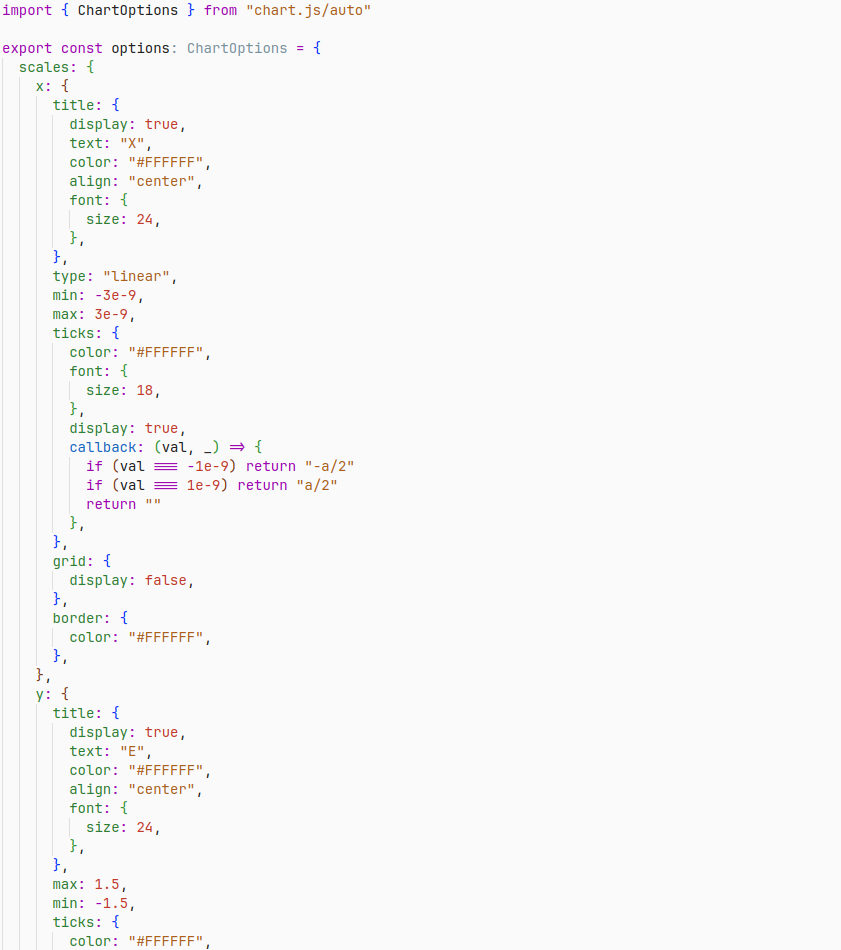
\includegraphics[width=\textwidth,height=\textheight,keepaspectratio]{options.png} 
	\caption{Początek pliku options.ts dla wykresu skończonej studni potencjału}
	\label{fig:options.ts}
	\end{figure}
	
	 W pliku data.ts znajdziemy jedną stałą, widoczną na rysunku \ref{fig:data.ts}, która określa ile szkiców funkcji ma pojawić się na wykresie, jak i współrzędne punktów. Dodatkowo znajdziemy w tym pliku kolory wykresów oraz ich opis w legendzie.
	
	\begin{figure}[H]
	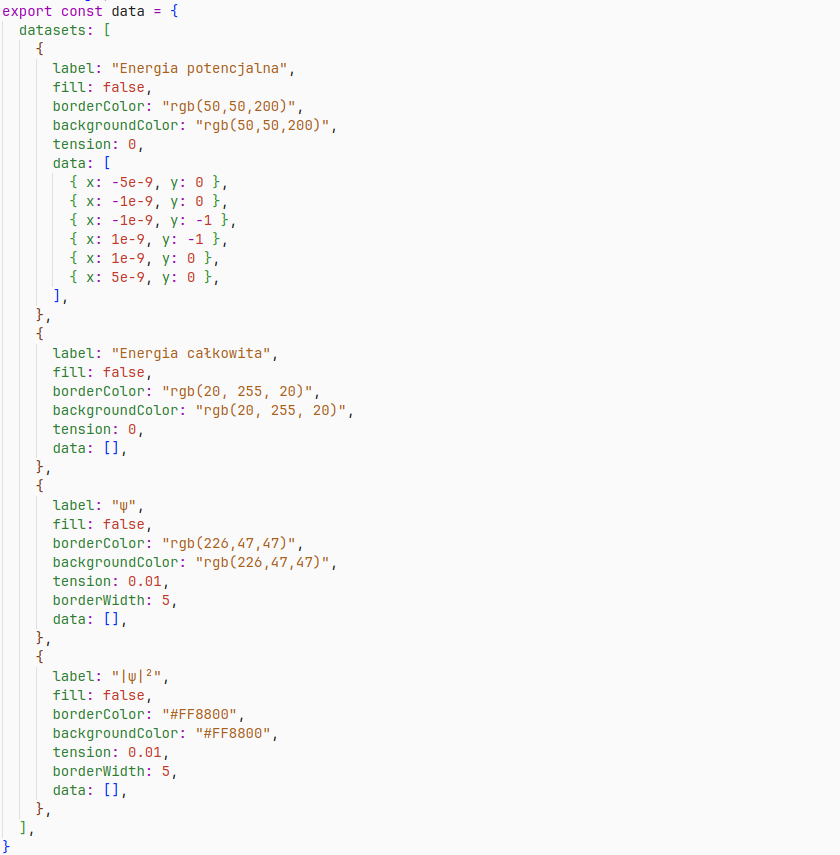
\includegraphics[width=\textwidth,height=\textheight,keepaspectratio]{data.png} 
	\caption{Plik data.ts dla wykresu skończonej studni potencjału}
	\label{fig:data.ts}
	\end{figure}
	
	W pliku chart.js importowane są stałe z dwóch poprzednich plików, w celu utworzenia wykresu, który to proces widać na rysunku \ref{fig:new-chart}. 
	
	\begin{figure}[H]
	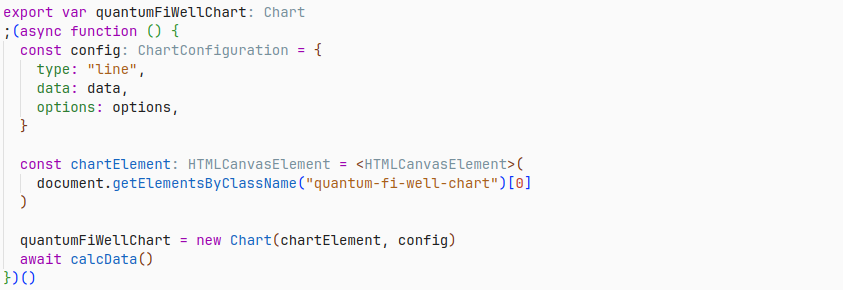
\includegraphics[width=\textwidth,height=\textheight,keepaspectratio]{new chart.png} 
	\caption{Tworzenie wykresu skończonej studni potencjału}
	\label{fig:new-chart}
	\end{figure}
	
	Poza tym znajduje się tutaj wybór elementu canvas, użytego do wyświetlenia wykresu, ale co ważniejsze wywołanie funkcji, do pozyskania danych, które mają być naniesione na wykres (rysunek \ref{fig:calc-data}). Proces ten został szerzej opisany w rozdziale 4.5. 
	
	\begin{figure}[H]
	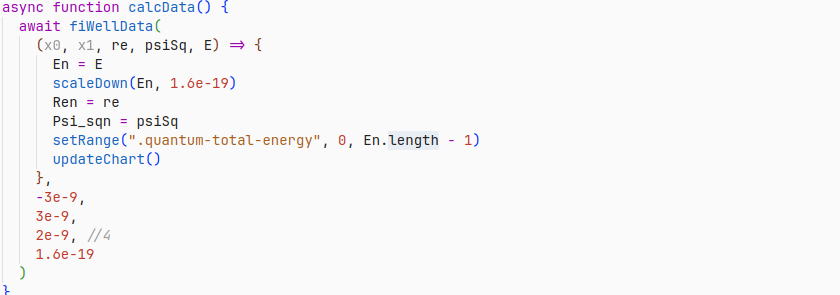
\includegraphics[width=\textwidth,height=\textheight,keepaspectratio]{calc data.png} 
	\caption{Wywołanie funkcji do obliczeń fizycznych i przedstawienia ich na wykresie}
	\label{fig:calc-data}
	\end{figure}
	
	Dodatkowo w pliku chart.js znajdują się wszelkie ustawienia do reagowania na przyciski i suwaki w aplikacji, przy pomocy wbudowanego wzorca projektowego obserwatora, co przedstawiłem na rysunkach \ref{fig:update-chart} i \ref{fig:slider-change}.
	
	\begin{figure}[H]
	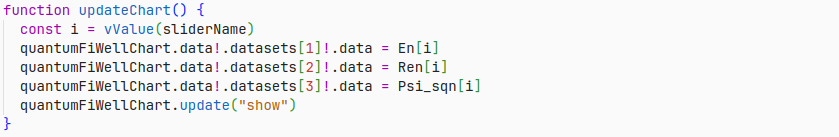
\includegraphics[width=\textwidth,height=\textheight,keepaspectratio]{update chart.png} 
	\caption{Funkcja do aktualizacji wykresu po wprowadzeniu zmian}
	\label{fig:update-chart}
	\end{figure}
	
	\begin{figure}[H]
	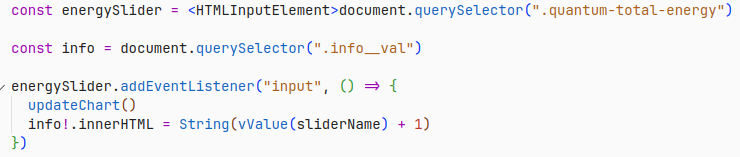
\includegraphics[width=\textwidth,height=\textheight,keepaspectratio]{slider change.png} 
	\caption{Kod odpowiedzialny za wywołanie aktualizacji wykresu po przesunięciu suwaka}
	\label{fig:slider-change}
	\end{figure}
	
	W projekcie znaleźć też można kilka plików, które ciężko przypisać do jakiejś konkretnej grupy. W pliku physics-constants.ts znajdują się wartości stałych fizycznych użytych w projekcie. Obecny jest również plik python-version-check.ts, odpowiedzialny za sprawdzanie obecności i wersji zainstalowanego interpretera Pythona oraz biblioteki NumPy.
	
	
	
	\section{Obliczenia fizyczne w Pythonie}
		Implementacja obliczeń zagadnień cząstki swobodnej, nieskończonej studni potencjału i progu potencjału, wymaga jedynie przepisania równań \ref{eqn:free-particle-gen-solution}, \ref{eqn:well-inside-sol} i \ref{eqn:potential-jump-solution} do Pythona, co nie wymaga dłuższego tłumaczenia.
		
		Sytuacja jest już odmienna dla pozostałych zagadnień, zaczynając od skończonej studni potencjału. Istnieją w niej bowiem, tak jak w studni nieskończonej, skwantowane stany energii dla cząstki związanej, jednak wyznaczenie ich nie wyraża się prostym wzorem. Jak jest wyjaśnione w \cite{wikipedia-well}, na podstawie wzorów \ref{eqn:k-fi-well}, \ref{eqn:gamma-fi-well}, \ref{eqn:fi-well-k-gamma} możemy zagadnienie skończonej studni, sprowadzić do jednej zmiennej $v$ :
		
		\begin{equation}\label{eqn:fi-well-vu}
			\sqrt{u_0^2-v^2} = 
			\left\{
		\begin{matrix}
			v\tan v \\ -v\cot v 
		\end{matrix}\right. ,
		\end{equation}
		
gdzie:
	\[u_0^2=\frac{ma^2V_0}{2\amshbar^2},\]
	\[v=\frac{ka}{2}.\]
		
Liczbę rozwiązań równania \ref{eqn:fi-well-vu} możemy wyznaczyć jako:

	\begin{equation}
	N = \left \lceil \frac{2u_0}{\pi} \right \rceil,
	\end{equation}
	
a każdego z nich należy szukać w przedziałach

	\begin{equation}\label{v-range}
	v_i \in \left< \frac{\pi}{2}(i-1), \; \frac{\pi}{2}i \right) \;\; \textrm{dla} \; \; i = 1, 2, ... N
	\end{equation}
	
	Ze względu na szybkość początkowo pomyślałem o zastosowaniu metody Newtona \cite{newton-method}, jednak metoda ta nie daje możliwości znalezienia miejsca zerowego w zadanym przedziale. Użyłem więc metody bisekcji \cite{bisection-method}, co przedstawiłem na rysunku \ref{fig:bisection}, a różnica czasu w wykonywaniu tych dwóch metod okazała się w moim przypadku marginalna.
		
	\begin{figure}[h]
		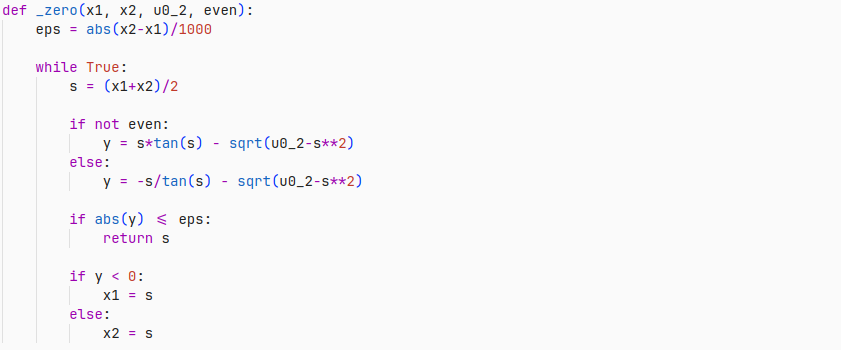
\includegraphics[width=\textwidth,height=\textheight,keepaspectratio]{bisection.png}
		\caption{Implementacja metody bisekcji}
		\label{fig:bisection}
	\end{figure}

Warto jednocześnie zaznaczyć, że wyjątkowej uwagi wymaga znalezienie ostatniego rozwiązania tj. $v_N$. Prawa granica przedziału \ref{v-range} może być na tyle oddalona od rozwiązania, że wartość ze środka tego przedziału, którą w pierwszej iteracji wybiera algorytm bisekcji, wyniesie więcej niż $u_0$, co spowoduje że w równaniu \ref{eqn:fi-well-vu} pierwiastkowana będzie liczba ujemna. Ponieważ szukane rozwiązania muszą być wartościami rzeczywistymi, przy ostatniej iteracji prawą granicę przedziału, w którym szukane jest miejsce zerowe, ustalam jako $u_0$, co można zobaczyć na rysunku \ref{fig:bisection2}.
	\begin{figure}[H]
		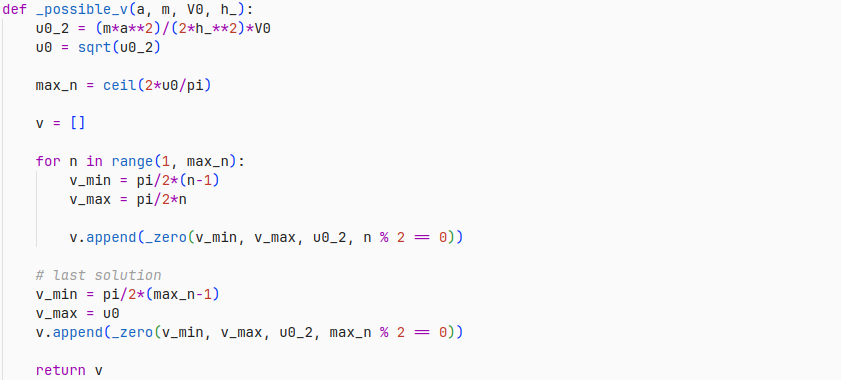
\includegraphics[width=\textwidth,height=\textheight,keepaspectratio]{bisection2.png} 
		\caption{Funkcja znajdująca wszystkie wartości $v$}
		\label{fig:bisection2}
	\end{figure}
	
	Kolejnym przypadkiem, wymagającym dodatkowej pracy, jest obliczenie stałych z układu równań \ref{eqn:barrier-system} dla bariery potencjału. Pomimo że jest to układ liniowy, mnogość wyrazów oraz dziedzina liczb zespolonych powodują, że wygodniej było mi go rozwiązać przy pomocy biblioteki NumPy, co przedstawiłem na rysunku \ref{fig:linalg-solve}
	
	\begin{figure}[H]
		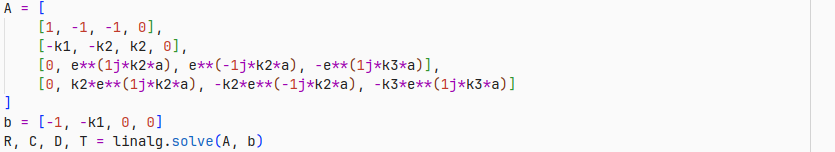
\includegraphics[width=\textwidth,height=\textheight,keepaspectratio]{linalg solve.png} 
		\caption{Implementacja numerycznego rozwiązania układu równań \ref{eqn:barrier-system}}
		\label{fig:linalg-solve}
	\end{figure}

		
	\section{Interfejs pomiędzy językiem TypeScript i Pythonem}
		Języki programowania tak odmienne jak TypeScript i Python uruchamiane są w zupełnie innych środowiskach. Framework Tauri daje tutaj wyjątkową możliwość obsługi języka TypeScript przy użyciu WebView \cite{tauri-arch}, a Pythona przy wykorzystaniu lokalnie zainstalowanego interpretera \cite{tauri-shell}.
		
		Problemem jest jednak przesyłanie danych między tymi językami, o czym nie myślano przy ich tworzeniu. Zastosowałem więc serializację danych do formatu JSON, który jest tekstową reprezentacją obiektu w języku TypeScript \cite{JS}. Wyniki obliczeń fizycznych są więc serializowane w Pythonie jedną z metod z rysunku \ref{fig:to-json}, czego przykład widać na rysunku \ref{fig:free-particle-py}. Dalej wyniki wysyłane są jako wyjście w powłoce systemowej i przekazywane przez Tauri do skryptu napisanego w języku TypeScript, co można zobaczyć na rysunku \ref{fig:ts-run-python}.
		
	\begin{figure}[H]
	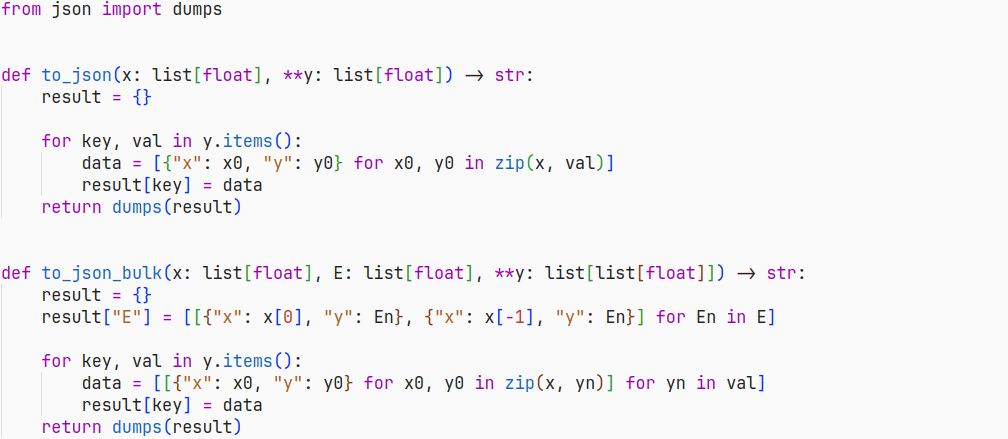
\includegraphics[width=\textwidth,height=\textheight,keepaspectratio]{to_json.png} 
	\caption{Kod z pliku json\_export.py}
	\label{fig:to-json}
	\end{figure}	
	
	\begin{figure}[H]
	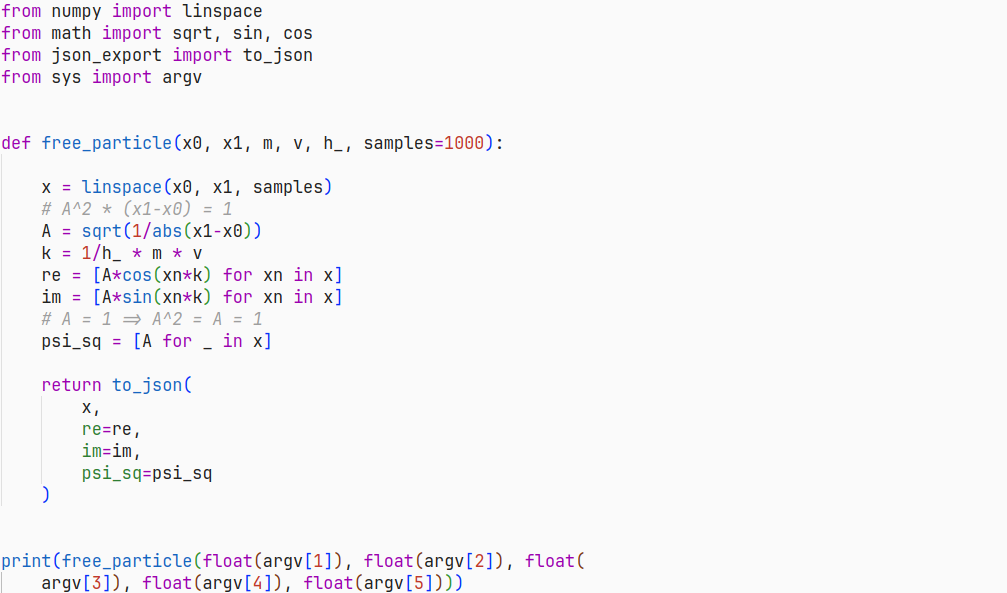
\includegraphics[width=\textwidth,height=\textheight,keepaspectratio]{free_particle py.png} 
	\caption{Wykorzystanie funkcji to\_json w pliku free\_particle.py}
	\label{fig:free-particle-py}
	\end{figure}
	
	\begin{figure}[H]
	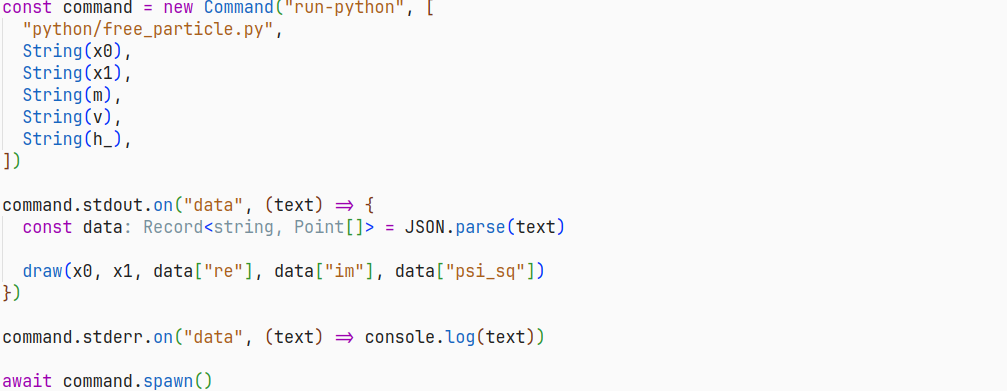
\includegraphics[width=\textwidth,height=\textheight,keepaspectratio]{ts run python.png} 
	\caption{Kod z pliku free-particle.ts}	
	\label{fig:ts-run-python}
	\end{figure}
	
	
	\section{Wdrożenie i dystrybucja aplikacji}
	Aplikacja została stworzona przy użyciu frameworka Tauri, który umożliwia kompilację do formatów .msi i .exe na system Windows, .deb i .AppImage na system GNU/Linux. Możliwa jest też kompilacja na system macOS na architekturę procesora x86 i ARM, jednak nie sprawdzałem tych opcji, ponieważ nie mam dostępu do takich urządzeń.
	
	Udostępnione przeze mnie zostały formaty .msi, który w przeciwieństwie do .exe jest dedykowany dla instalatorów programów na system Windows oraz .deb, ponieważ jest to format wspierany przez największe dystrybucje systemu GNU/Linux, czyli Debian i Ubuntu. Dodatkowo format .AppImage powodował problem szerzej opisany w kolejnym rozdziale. 
	
	Framework Tauri sam kopiuje do wersji skompilowanej niezbędne pliki .html, .css .ts oraz wszelkie obrazy i fonty użyte w plikach .css, jednak użyte skrypty .py muszą być specjalnie oznaczone jako zasób aplikacji w pliku konfiguracyjnym tauri.conf.json. Ponieważ twórcy frameworka Tauri stworzyli go z myślą o bezpieczeństwie \cite{about-tauri}, w pliku konfiguracyjnym zadeklarować, żeby aplikacja miała możliwość wykonywania poleceń systemowych, do uruchomienia interpretera Pythona oraz możliwość odczytu plików, do użycia plików ze skryptami Pythona.
	
	Ponieważ obliczenia matematyczne wykonywane są przy użyciu języka Python, niezbędny do działania aplikacji jest zainstalowany interpreter Pythona 3.11 lub nowszy z zainstalowanym modułem NumPy. Zdecydowałem się nie dołączać interpretera do instalatora mojej aplikacji, ponieważ znacząco zwiększyłoby to rozmiar finalnego pliku. 
	\section{Problemy, ograniczenia i możliwości rozwoju}
	Jedno z ważniejszych ograniczenie mojej aplikacji leży w interfejsie pomiędzy językiem TypeScript i Pythonem. O ile wykonanie samych obliczeń fizycznych w Pythonie liczyć można w milisekundach, to proces zserializowania danych, czyli zamiany ich na tekst, przekazania ich do odczytu i deserializacji, czyli zamiany tekstu na obiekt, w języku TypeScript wydłuża ten proces do kilkuset milisekund, zwykle co najmniej 200. Jest to czas niezauważalny, jeżeli potrzebne jest wykonanie obliczeń raz lub stosunkowo rzadko, co ma miejsce w aplikacji, jednak częste odświeżanie wyświetlanych danych byłoby po prostu niemożliwe do zrealizowania przy zastosowanym rozwiązaniu. Należy jednocześnie zwrócić uwagę, że przy bardziej rozbudowanych scenariuszach fizycznych czas przekazywania danych może okazać się nieznaczący, jeśli samo wykonywanie obliczeń fizycznych trwać znacznie dłużej. Dokładnie takie przypadki miałem na względzie, decydując o zastosowaniu Pythona w projekcie i jest to kierunek, w którym aplikacja mogłaby zostać w przyszłości rozwinięta.
	
	Kolejną rzeczą, która ogranicza aplikację jest forma dystrybucji. Na przestrzeni lat aplikacje desktopowe ustępowały popularnością aplikacjom webowym. W wyniku takich zmian użytkownicy przyzwyczajeni do korzystania z przeglądarki internetowej mogą nie chcieć poświęcić czasu na pobranie i zainstalowanie mojej aplikacji. Niestety jednak, pomimo że jest to już możliwe, wykonywanie skryptów Pythona w przeglądarce jest dalej w fazie rozwoju \cite{python-webassembly}, co wymusza taką formę aplikacji.
	
	Z pozoru największym problemem, jaki napotkałem, był fakt, że aplikacja po skompilowaniu do formatu .AppImage nie była w stanie poprawnie wywoływać skryptów Pythona. Jak jednak powiedziałem, problem tylko z pozoru wydał się krytyczny, a to przez fakt, że formaty .deb i .msi nie sprawiały żadnych problemów. Wciąż zaintrygowany tym nieoczekiwanym zachowaniem, zgłosiłem się przez komunikator Discord o pomoc do zespołu wsparcia frameworka Tauri. Okazało się, że nie jest to spodziewane zachowanie i najprawdopodobniej napotkałem błąd w samym frameworku. Na prośbę zespołu wsparcia zamieściłem repozytorium z minimalnym kodem niezbędnym do odtworzenia tego błędu \cite{app-error-repo}.
	
	Ważnym aspektem, który niekiedy spowalniał tworzenie pracy, jest fakt że framework Tauri, wydany w 2022 roku \cite{tauri-release}, jest stosunkowo nową technologią. Pomimo że dostępną jest dokumentacja, to potrafi ona zawierać braki lub niedopowiedzenia, a szukanie szczegółowych odpowiedzi może stanowić wyzwanie, ponieważ nie istnieje na ten temat znacząca ilość literatury.
	

\chapter{Interfejs aplikacji}
	Przy projektowaniu interfejsu najbardziej zależało mi na przejrzystości i intuicyjności. Były to wskaźniki dla mnie najważniejsze, ponieważ chciałem, aby użytkownik mógł szybko przystąpić do korzystania z aplikacji i nauki trudnej dziedziny, jaką jest mechanika kwantowa. Dzięki prostemu interfejsowi w aplikacji nie musiałem udzielać instrukcji, jak ją nawigować i z niej korzystać, co mogłoby odstraszyć potencjalnego użytkownika.
	\section{Ekran główny i nawigacja}
	Po włączeniu aplikacji jako pierwszy zobaczymy ekran główny widoczny na rysunku  \ref{fig:main-page}. Umieściłem na nim krótką informację o celu stworzenia aplikacji i jej zawartości, a także zamieściłem link do kodu aplikacji. Poniżej tych informacji zamieściłem również element pokazujący, czy użytkownik ma zainstalowany interpreter Pythona w odpowiedniej wersji oraz bibliotekę NumPy.
	
	\begin{figure}[H]
	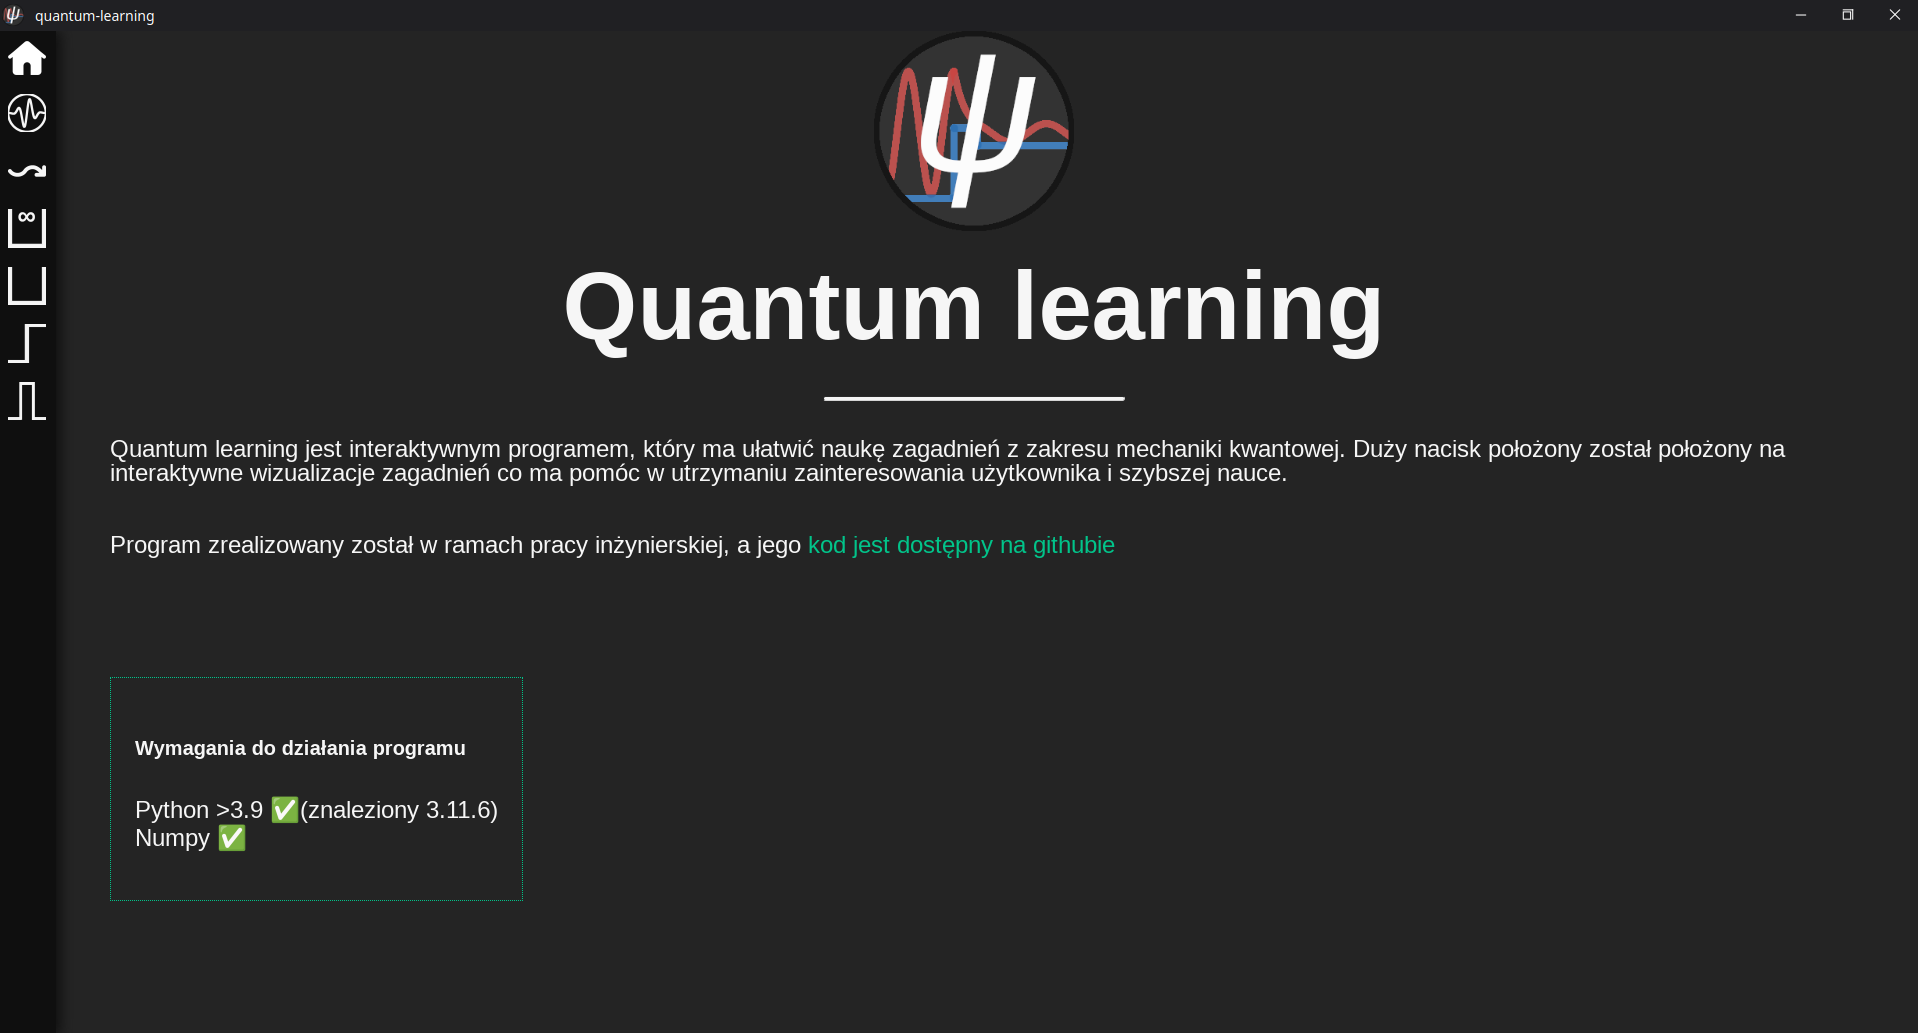
\includegraphics[width=\textwidth,height=\textheight,keepaspectratio]{main page.png} 
	\caption{Ekran główny}
	\label{fig:main-page}
	\end{figure}
	
	Do nawigacji po rozdziałach w aplikacji użytkownik może użyć menu po lewej stronie. Nieaktywne menu składa się tylko z prostych ikon, jednak po najechaniu kursorem pokazują się pełne nazwy rozdziałów co widać na rysunku \ref{fig:menu-unfolded}. Nazwa rozdziału po najechaniu kursorem podświetla się innym kolorem, a jej kliknięcie przenosi użytkownika do danego tematu.
	
	\begin{figure}[H]
	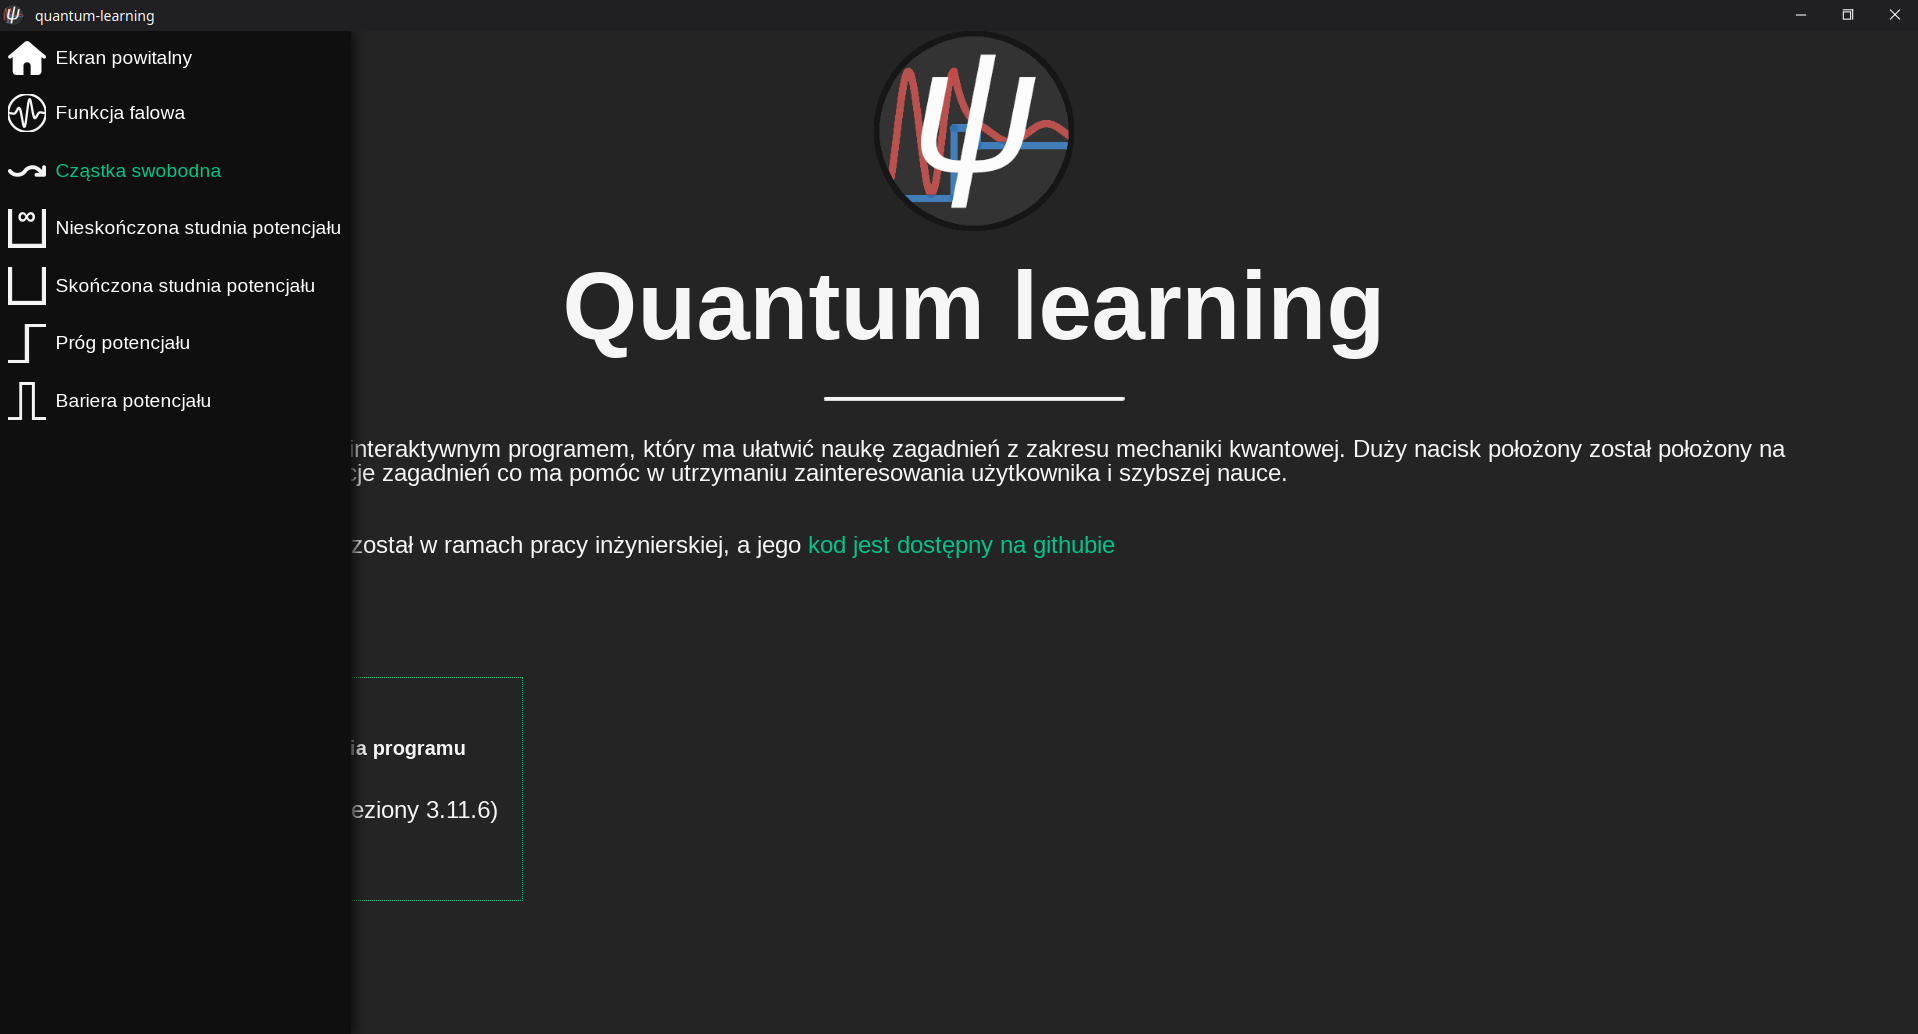
\includegraphics[width=\textwidth,height=\textheight,keepaspectratio]{menu unfolded.png} 
	\caption{Rozwinięte menu do nawigacji}
	\label{fig:menu-unfolded}
	\end{figure}
	
	\section{Interaktywna wizualizacja}
	Najwięcej uwagi w aplikacji przykuwają interaktywne wizualizacje omawianych zagadnień, co można zobaczyć na rysunku \ref{fig:free-chart}. Do każdego z rozwiązań równania Schrödingera przytoczonego w rozdziale 1.2 przygotowana została wizualizacja, przedstawiająca zachowanie funkcji falowej. W każdej z tych wizualizacji użytkownik ma możliwość wprowadzenia zmian niektórych parametrów oraz podglądu, jak zmieni się funkcja falowa w reakcji na te zmiany.
	
	\begin{figure}[H]
	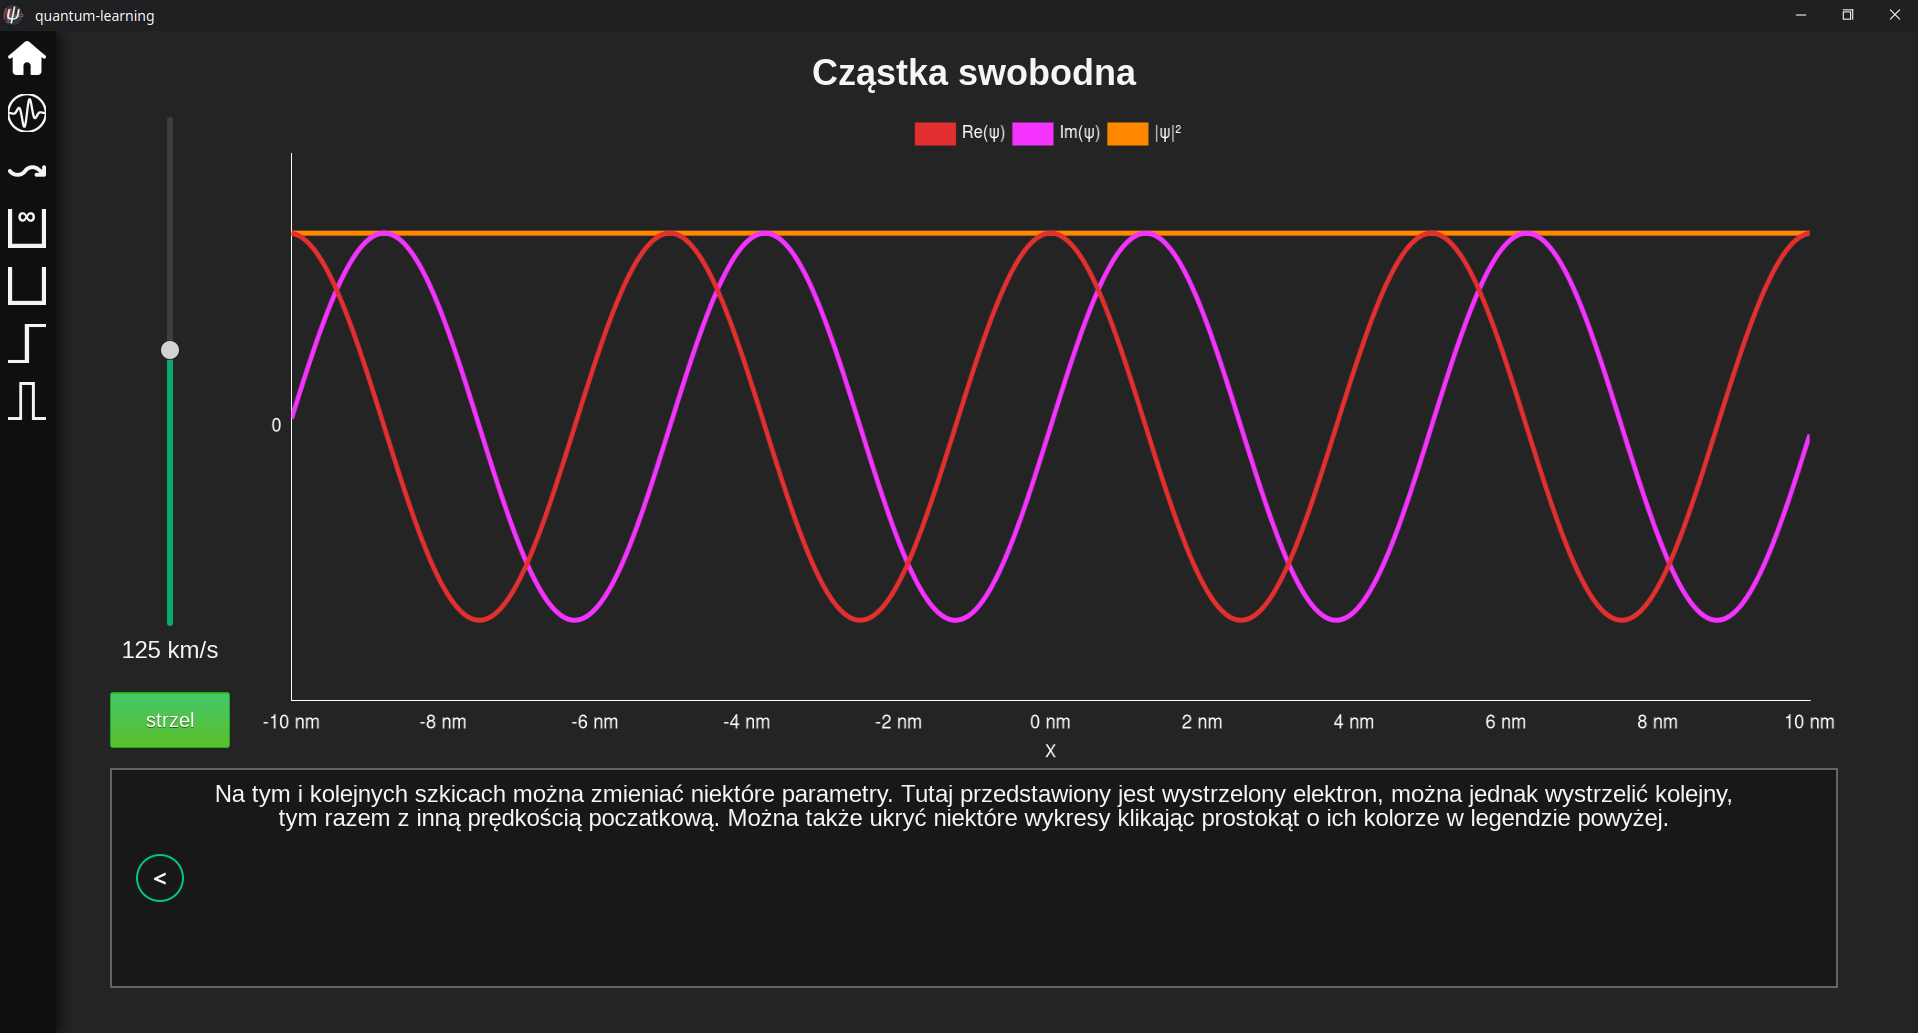
\includegraphics[width=\textwidth,height=\textheight,keepaspectratio]{free.png} 
	\caption{Widok rozdziału cząstka swobodna}
	\label{fig:free-chart}
	\end{figure}	
	
	Zaczynając od przypadku cząstki swobodnej, widocznego na rysunku \ref{fig:free-chart}, naszkicowana została funkcja falowa wraz z kwadratem jej modułu, czyli gęstością prawdopodobieństwa znalezienia cząstki w danym obszarze. Ponieważ funkcja falowa przyjmuje wartości zespolone, oddzielnie zostały naszkicowane część rzeczywista i urojona. Po lewej stronie znajduję się suwak, za pomocą którego użytkownik może wystrzelić elektron o prędkości z przedziału 20 km/s - 250 km/s i zobaczyć, jak zmieni się kształt funkcji falowej. Amplituda funkcji falowej została ustalona jako 1, co dla opisanej na osi x skali oznacza, że gęstość prawdopodobieństwa $|\psi|^2$ jest nieprawidłowo unormowana. Zdecydowałem się na taki zabieg, aby uniknąć znacznych rozbieżności między wartościami $\psi$ oraz $|\psi|^2$ co utrudniłoby przedstawienie ich na tym samym wykresie. Dodatkowo poprawna normalizacja nie była konieczna do opisu tego przypadku. 
	
	Kolejna wizualizacja poświęcona jest cząstce w nieskończonej studni potencjału. Zgodnie ze wzorem \ref{eqn:discrete-well} wiadomo, że cząstka przyjmuje dyskretne wartości energii, więc dołączony został suwak do zmiany numeru stanu energetycznego $n$. W przypadku studni potencjału funkcja falowa przyjmuje wartości czysto rzeczywiste lub czysto urojone nie było więc sensu rozdzielać tych wartości w legendzie i przedstawione one są zbiorczo jako $\psi$, co widać na rysunku \ref{fig:inf-well}. Dodatkowo ukazana została wartość energii każdego stanu.
	
	\begin{figure}[H]
		\subfloat[$\psi$]{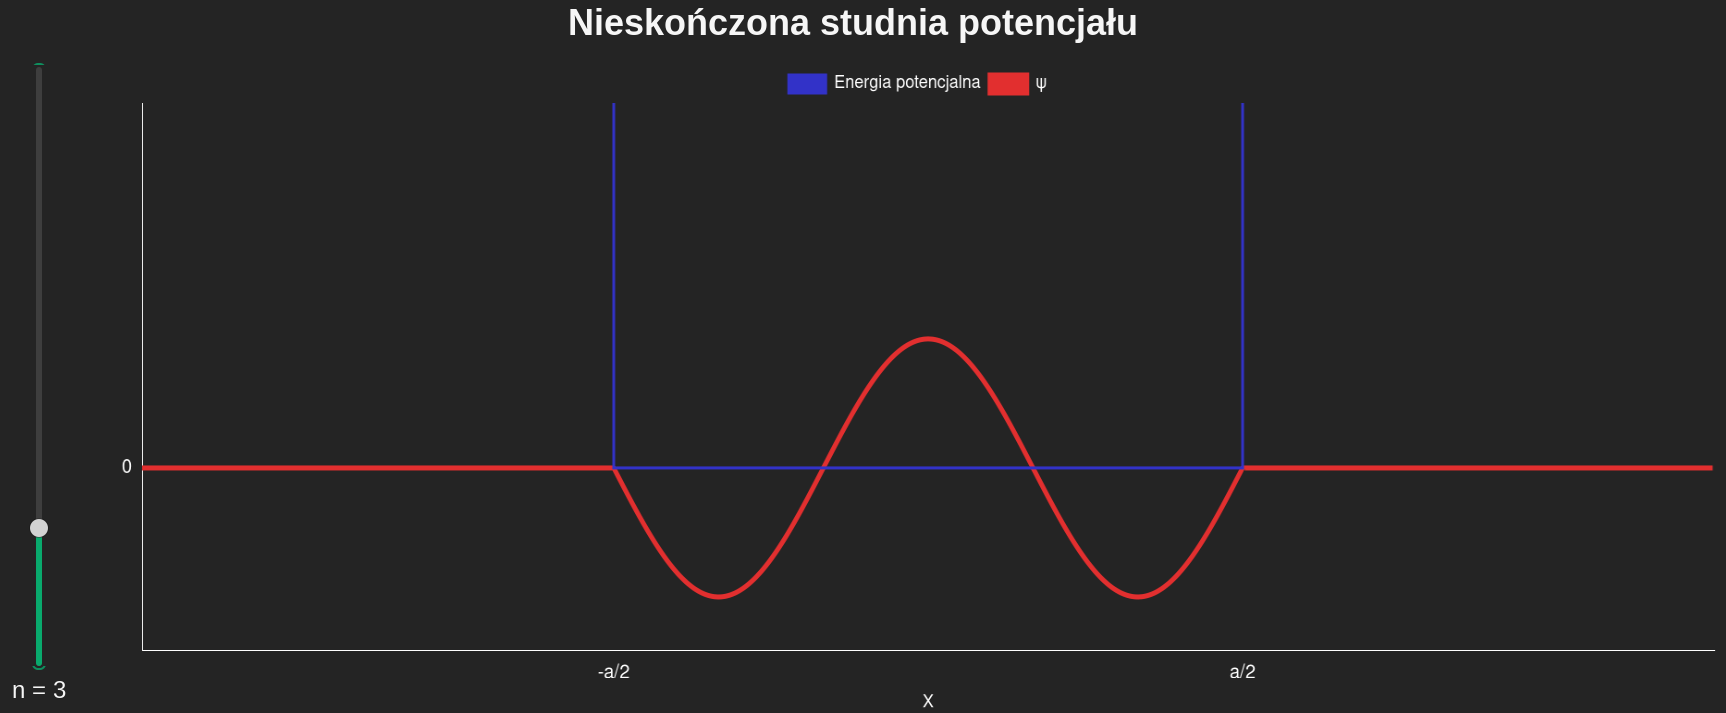
\includegraphics[width=\textwidth,height=\textheight,keepaspectratio]{infwell1.png}}\\
		\subfloat[$|\psi|^2$]{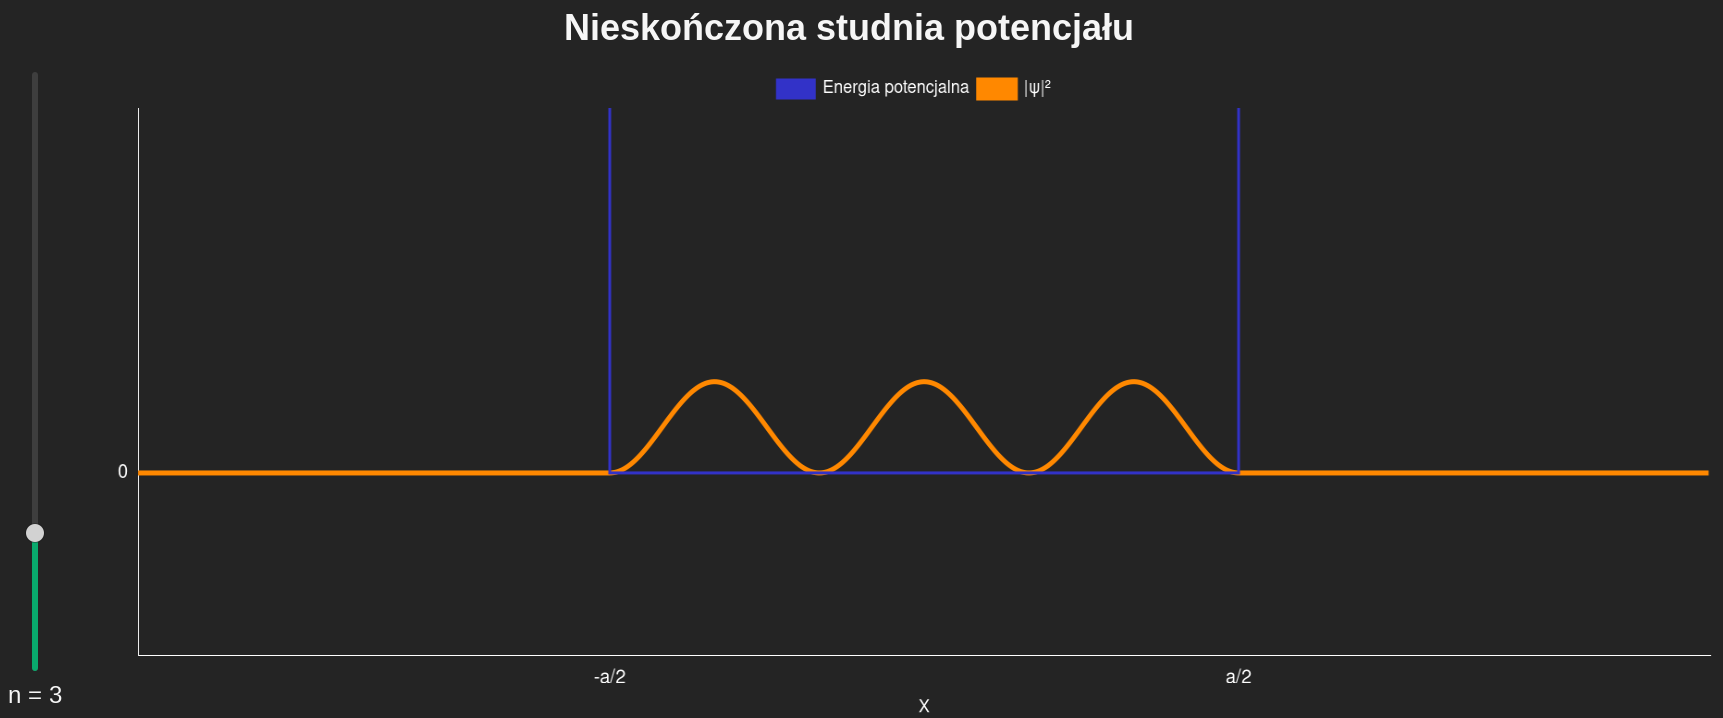
\includegraphics[width=\textwidth/2,height=\textheight,keepaspectratio]{infwell2.png}}
		\subfloat[Energia]{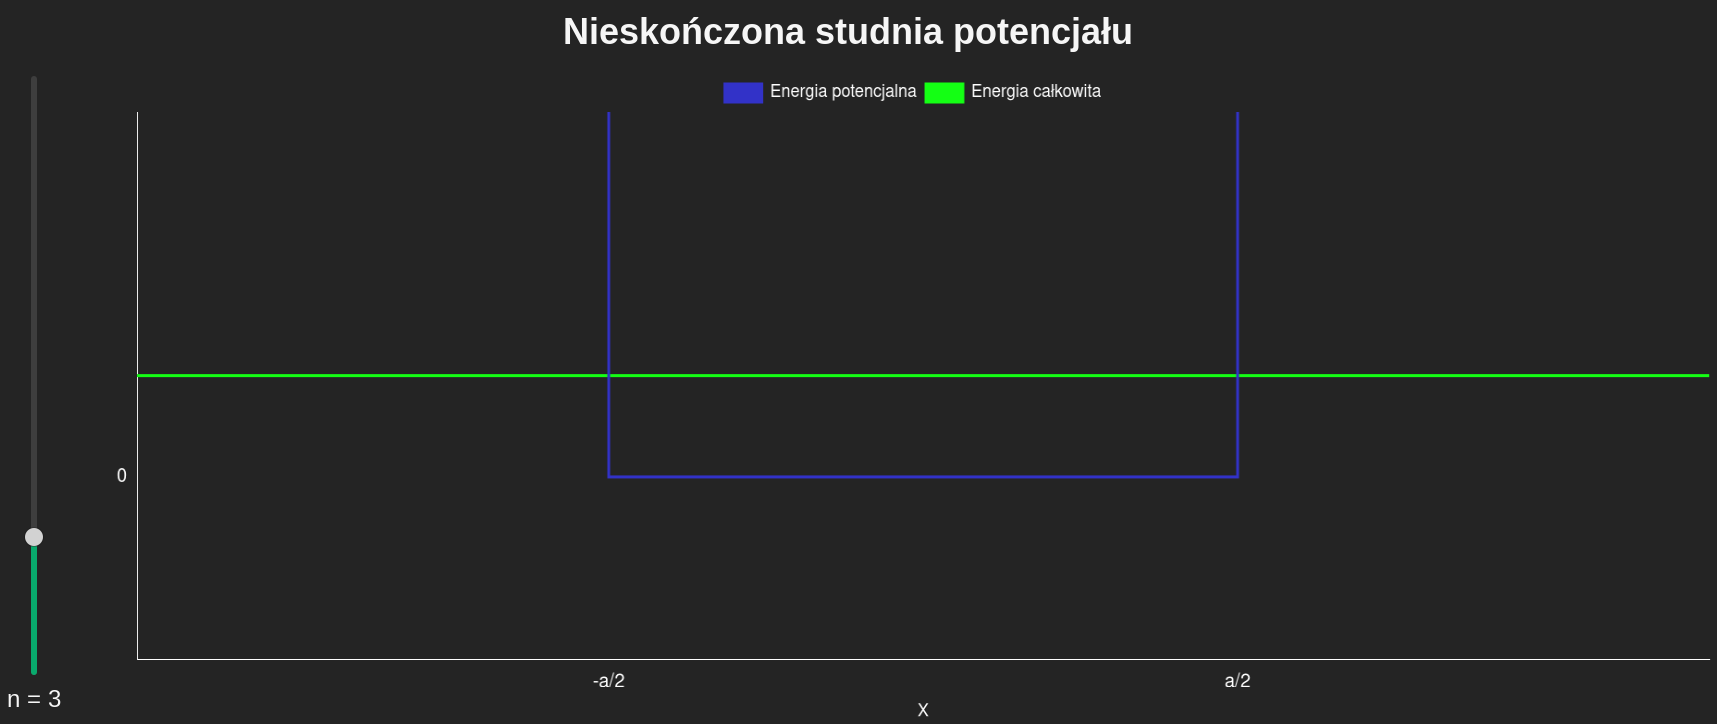
\includegraphics[width=\textwidth/2,height=\textheight,keepaspectratio]{infwell3.png}}
		\caption{Wizualizacja z rozdziału nieskończona studnia potencjału}
		\label{fig:inf-well}
	\end{figure}
	
	Bardzo podobnie prezentuje się wizualizacja skończonej studni potencjału przedstawiony na rysunku \ref{fig:fi-well}, jednak w tym przypadku zdecydowałem się nanieść wszystkie wartości na jeden wykres. Przez ograniczoną głębokość studni wartości energii nie wykraczają ponad wykres, w przeciwieństwie do większych wartości $n$ w studni nieskończonej.
	
	\begin{figure}[H]
	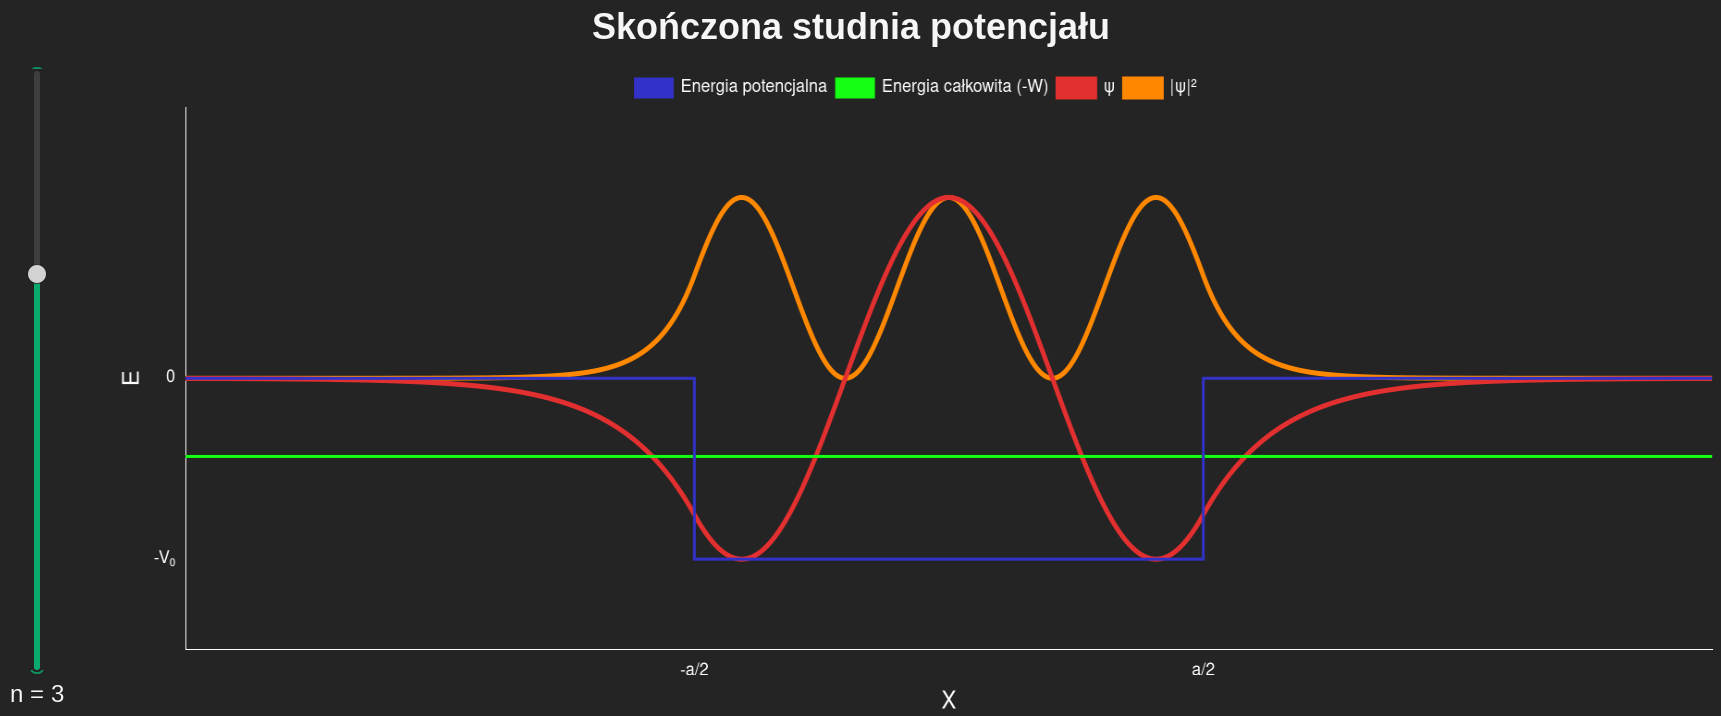
\includegraphics[width=\textwidth,height=\textheight,keepaspectratio]{fiwell.png} 
	\caption{Wizualizacja z rozdziału skończona studnia potencjału}
	\label{fig:fi-well}
	\end{figure}
	
	Dla progu potencjału, tak jak w przypadku cząstki swobodnej, oddzielnie naszkicowane zostały części rzeczywista i urojona funkcji falowej. Do dyspozycji użytkownika jest suwak widoczny na rysunku \ref{fig:potential-jump}, służący do zmiany energii wystrzelonej cząstki. Szkic wartości tej energii oznaczony został kolorem zielonym i reaguje swoją pozycją na zmiany wprowadzone suwakiem. Suwak uniemożliwia ustawienie przypadku, gdy $E=V_0$, ponieważ wymagałby on dodatkowej implementacji, a i tak jest on najczęściej pomijany w podręcznikach \cite{fiz atom} \cite{mechanika kwant} \cite{fiz kwant}.
	
	\begin{figure}[H]
	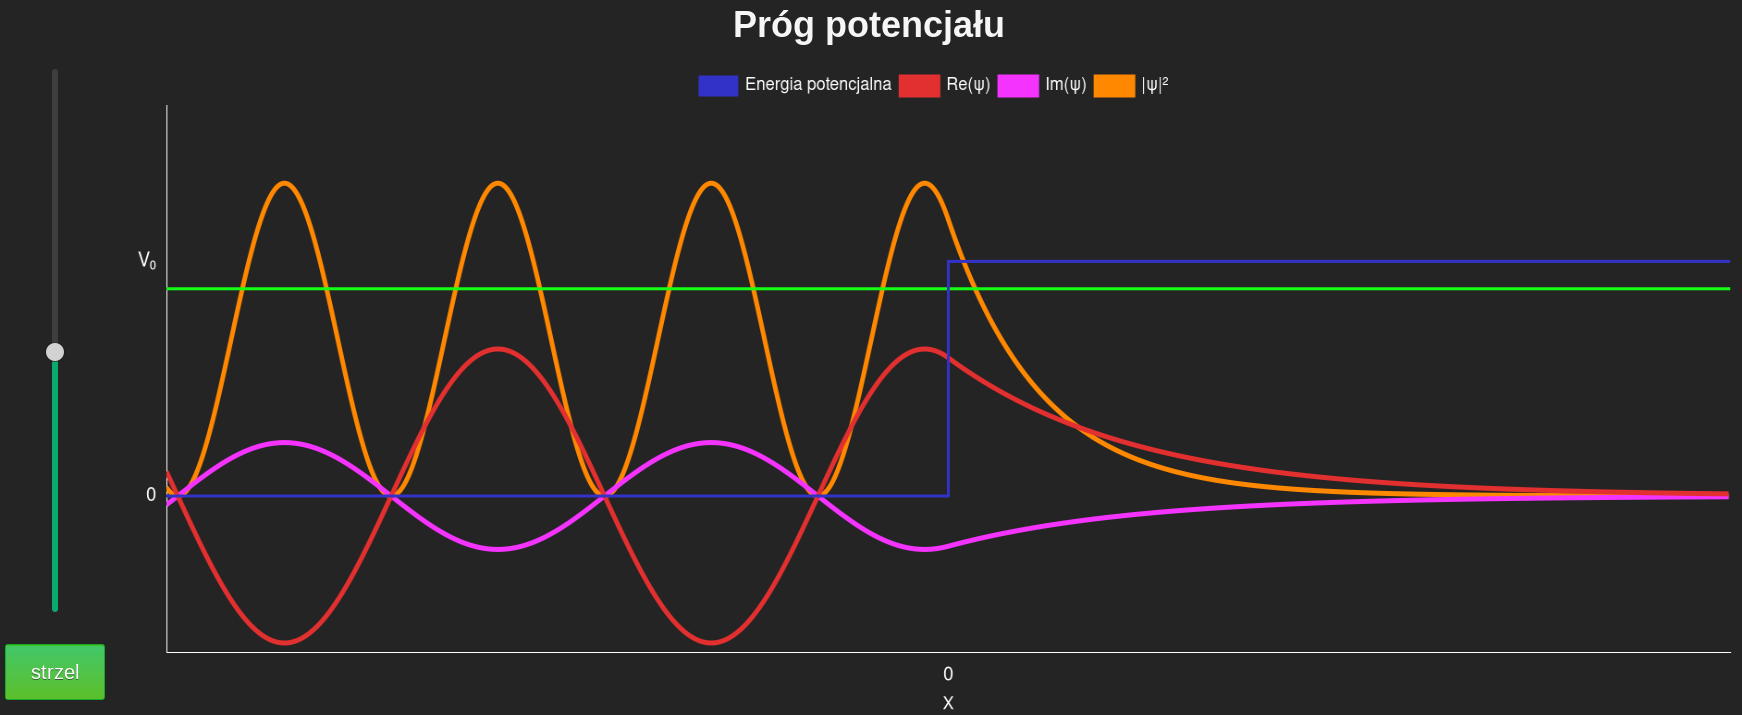
\includegraphics[width=\textwidth,height=\textheight,keepaspectratio]{jump.png} 
	\caption{Wizualizacja z rozdziału próg potencjału}
	\label{fig:potential-jump}
	\end{figure}
	
	Dosyć zbliżona do wizualizacji progu potencjału jest zasada działania wizualizacji bariery potencjału, widoczna na rysunku \ref{fig:potential-barrier}. Tak samo dostępny jest suwak do zmiany wartości wystrzelonej cząstki, uniemożliwiający ustawienie $E=V_0$.
	
	\begin{figure}[H]
	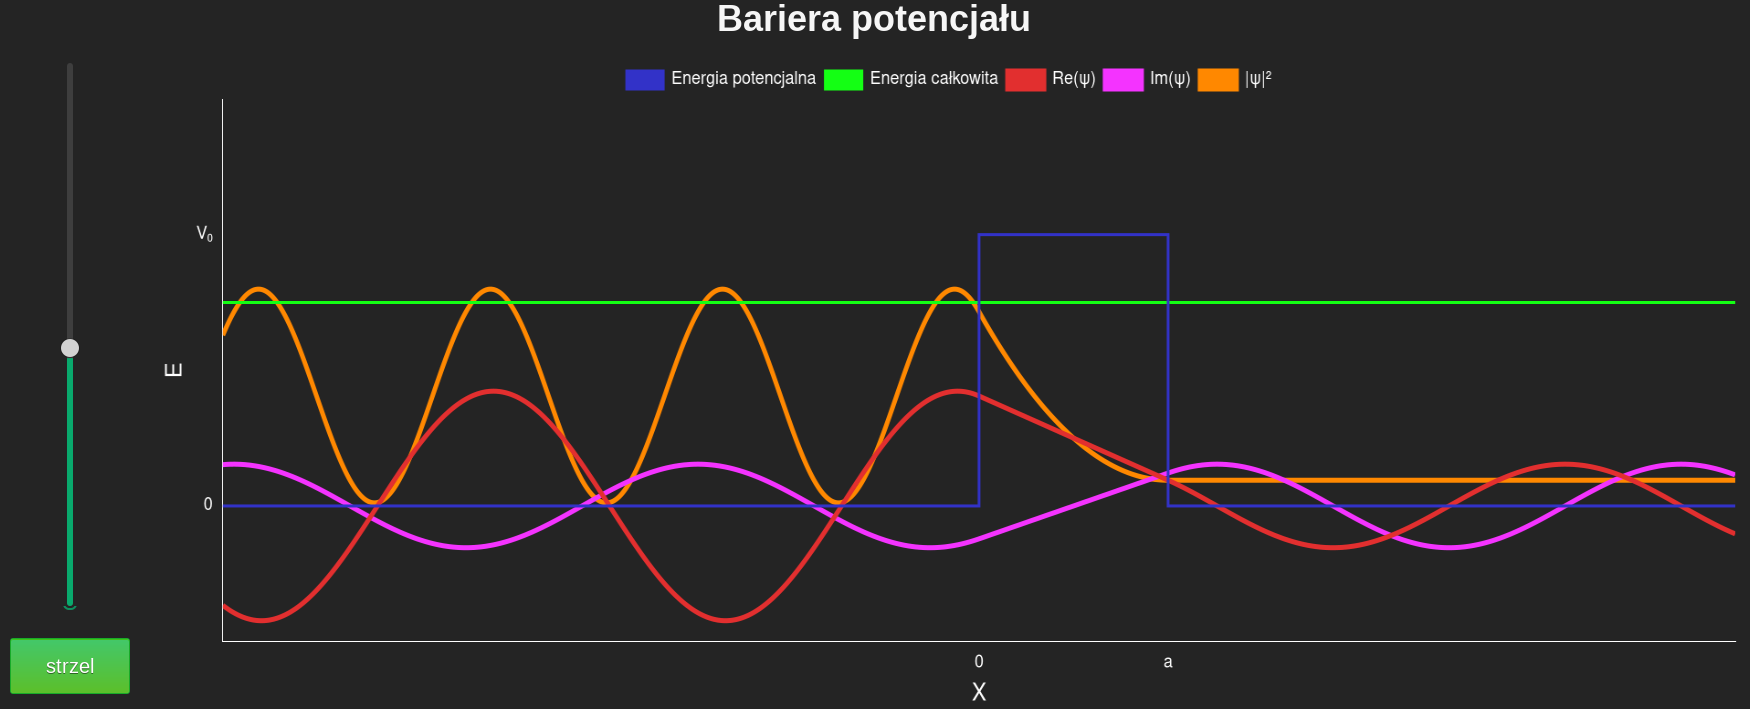
\includegraphics[width=\textwidth,height=\textheight,keepaspectratio]{barrier.png} 
	\caption{Wizualizacja z rozdziału bariera potencjału}
	\label{fig:potential-barrier}
	\end{figure}
	
	\section{Narrator}
	Zastosowane wizualizacje, pomimo że interesujące, wymagają opisu do wyjaśnienia i pełnego ich zrozumienia. Nie chciałem użytkownika przytłoczyć duża ilością tekstu oraz chciałem, aby wizualizacje stanowiły centralny punkt aplikacji. Jako rozwiązanie tych problemów, pod każdym szkicem zamieściłem okno, w którym tłumaczone są kolejne kroki prowadzące do znalezienia funkcji falowej dla danego scenariusza. Okno to, widoczne na rysunku \ref{fig:narrator}, składa się również z przycisków do nawigacji po kolejnych krokach. Dodatkowo wizualizacja nie jest niezależna od takiego narratora, a zamiast tego pokazywane są użytkownikowi elementy, które są akurat tłumaczone. Widać to zachowanie na rysunku \ref{fig:narrator}, gdzie przy tłumaczeniu wykresu funkcji falowej, tylko ta funkcja zostaje akurat pokazana.
	
	\begin{figure}[H]
	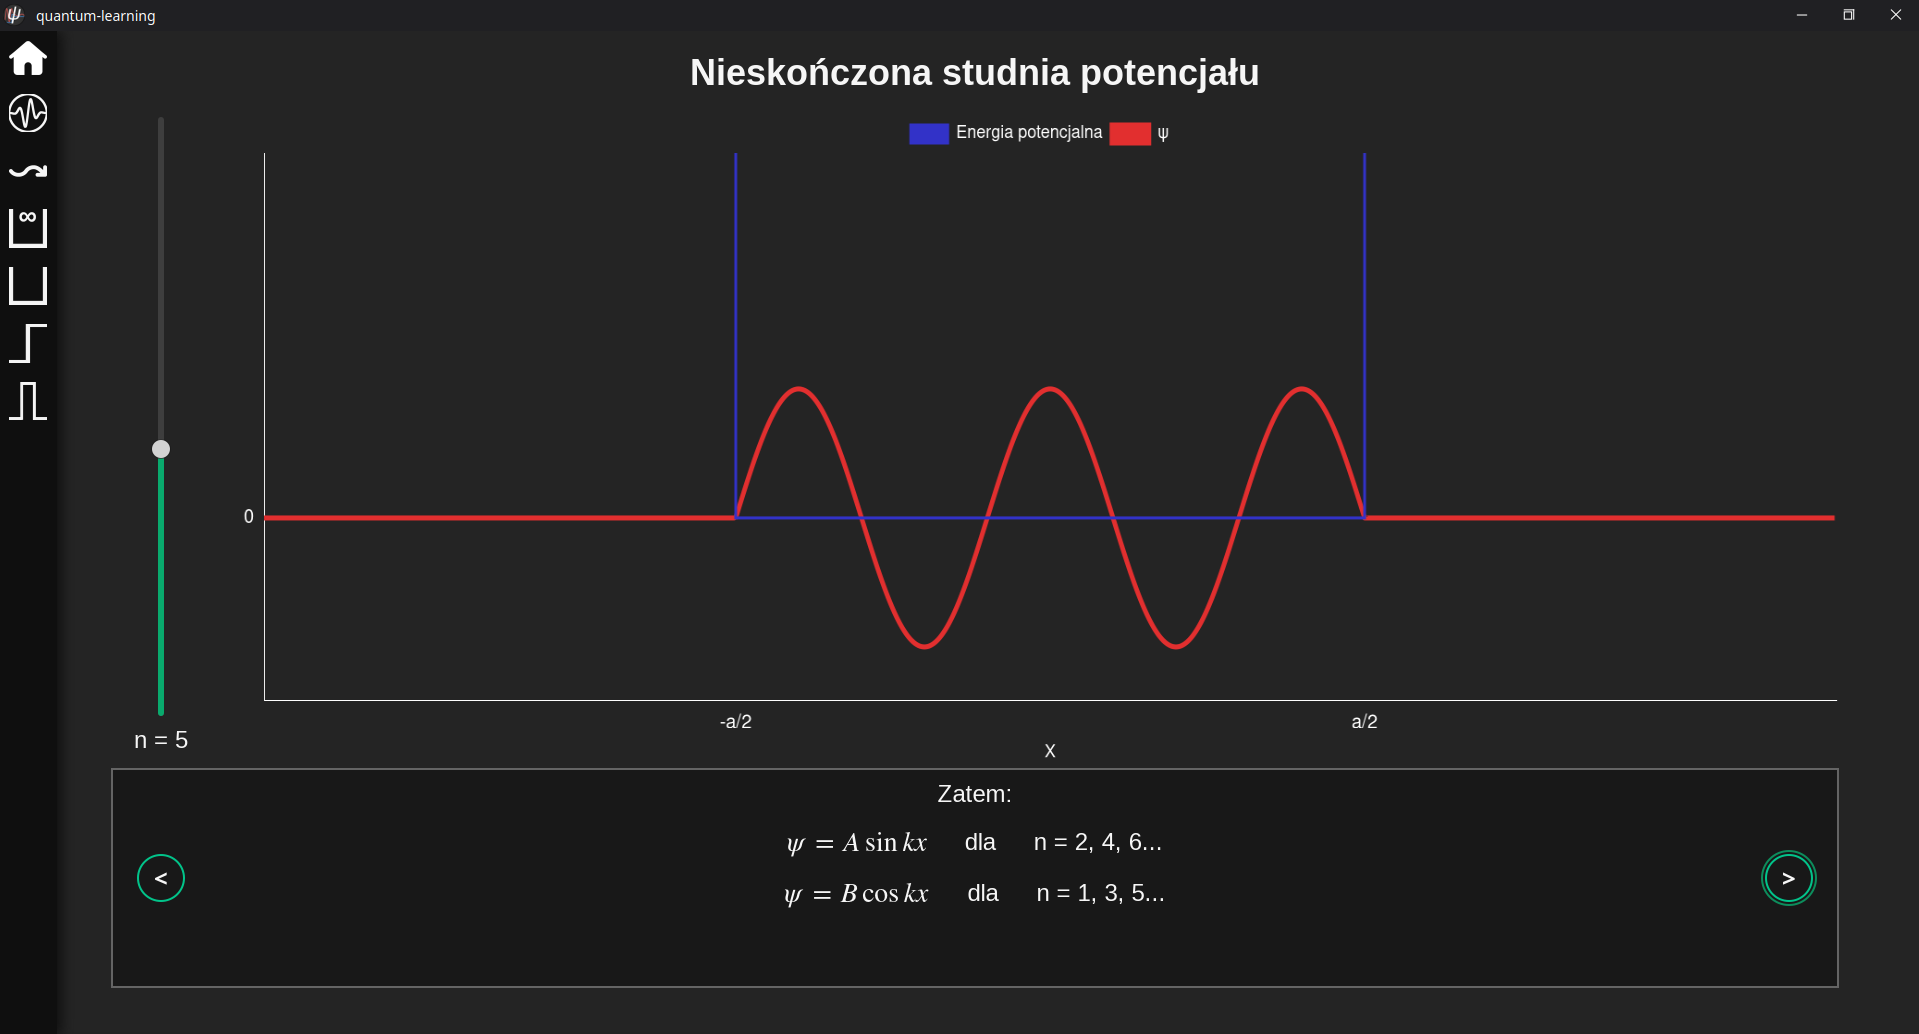
\includegraphics[width=\textwidth,height=\textheight,keepaspectratio]{narrator.png} 
	\caption{Funkcja falowa w nieskończonej studni potencjału}
	\label{fig:narrator}
	\end{figure}
	
\chapter{Podsumowanie i wnioski}
	Patrząc na stworzoną aplikację, uważam że początkowy cel został zrealizowany. Aplikacja zawiera typowe rozwiązania równania Schrödingera, a przy tym przedstawia te rozwiązania w ciekawy i przykuwający uwagę sposób. Można jej użyć do łatwiejszej nauki trudnych problemów mechaniki kwantowej, jednocześnie przedstawiając je w interesujący sposób. Należy oczywiście pamiętać, że aplikacja nie przedstawia każdego szczegółu zagadnień, a jedynie zbiera najważniejsze informacje na dane tematy.
	
	Dzięki zastosowanym technologiom możliwa jest rozbudowa aplikacji o kolejne przykłady. HTML, CSS, TypeScript i Python to bardzo popularne języki, dzięki czemu wiele osób poza mną byłoby w stanie dodać inne scenariusze do rozwiązania równania Schrödingera. Python daje też dużo elastyczności do wykonywania obliczeń fizycznych i symbolicznych, więc można niewątpliwe wyjść poza tematy opracowane przeze mnie.
	
	Najbardziej ograniczającą cechą aplikacji, o której nie można zapomnieć przy planowaniu jej rozwoju, jest stosunkowo długi czas przekazywania obliczonych danych pomiędzy językami TypeScript i Python. Mając to na uwadze, tworzone wizualizacje nie mogą być zbyt dynamiczne, albo odbywać się w czasie rzeczywistym. Bardzo dobrze jednak sprawdzą się wizualizacje mniej zmienne, ale wymagające więcej czasu na obliczenie.


\begin{thebibliography}{9}
	\bibitem{nuclear-stats}
	Statystyki eurostat na temat energetyki jądrowej, 
	\textit{https://ec.europa.eu/eurostat/statistics-explained/index.php?title=Nuclear\_energy\_statistics}
	(ostatni dostęp 28.04.2024)

	\bibitem{fiz atom}
	M.R. Wehre, H.A. Enge, J.A. Richards,
	\textit{Wstęp do fizyki atomowej}, 
	Państwowe Wydawnictwo Naukowe, Warszawa 1983. ISBN 83-01-02200-0
	
	\bibitem{mechanika kwant}
	L.D. Landau, E.M. Lifszyc,
	\textit{Mechanika kwantowa Teoria nierelatywistyczna}
	Państwowe Wydawnictwo Naukowe, Warszawa 1979. ISBN 83-01-00501-7
	
	\bibitem{fiz kwant}
	R. Eisberg, R. Resnick,
	\textit{Fizyka kwantowa atomów, cząsteczek, ciał stałych, jąder i cząstek elementarnych}
	Państwowe Wydawnictwo Naukowe, Warszawa 1983. ISBN 83-01-04350-1
	
	\bibitem{mozilla-HTML}
	Dokumentacja języka HTML,
	\textit{https://developer.mozilla.org/en-US/docs/Web/HTML}
	(ostatni dostęp 9.05.2024)
	
	\bibitem{mozilla-CSS}
	Dokumentacja języka CSS,
	\textit{https://developer.mozilla.org/en-US/docs/Web/CSS}
	(ostatni dostęp 9.05.2024)
	
	\bibitem{React}
	Strona biblioteki React,
	\textit{https://react.dev/}
	(ostatni dostęp 9.05.2024)
	
	\bibitem{Angular}
	Strona frameworka Angular,
	\textit{https://angular.io/}
	(ostatni dostęp 9.05.2024)
	
	\bibitem{Vue}
	Strona frameworka Vue.js,
	\textit{https://vuejs.org/}
	(ostatni dostęp 9.05.2024)
	
	\bibitem{Svelte}
	Strona frameworka Svelte,
	\textit{https://svelte.dev/}
	(ostatni dostęp 9.05.2024)
	
	\bibitem{TS}
	Typy w języku TypeScript,
	\textit{https://www.typescriptlang.org/docs/handbook/2/basic-types.html}
	(ostatni dostęp 9.05.2024)
	
	\bibitem{chartjs}
	Dokumentacja Chart.js, 
	\textit{https://www.chartjs.org/docs/latest/}
	(ostatni dostep 30.04.2024)
	
	\bibitem{mathjax}
	Dokumentacja MathJax,
	\textit{https://docs.mathjax.org/en/latest/}
	(ostatni dostep 30.04.2024)
	
	\bibitem{Python}
	Wes McKinney, 
	\textit{Python for Data Analysis}
	O'Reilly Media, 2012. ISBN 078-1-449-31979-3
	
	\bibitem{sympy}
	Dokumentacja SymPy, 
	\textit{https://docs.sympy.org/latest/index.html}
	(ostatni dostęp 13.01.2024)
	
	\bibitem{python-webassembly}
	Repozytorium Pyodide, 
	\textit{https://github.com/pyodide/pyodide}
	(ostatni dostęp 28.04.2024)
	
	\bibitem{wasm}
	Strona główna WebAssembly,
	\textit{https://webassembly.org/}
	(ostatni dostęp 9.05.2024)
	
	\bibitem{liczby zespolone}
	Liczby zespolone,
	\textit{https://en.wikipedia.org/wiki/Complex\_number}
	(ostatni dostęp 09.05.2024)
	
	\bibitem{lewis}
	Gilbert Lewis, 
	\textit{https://pl.wikipedia.org/wiki/Gilbert\_Lewis}
	(ostatni dostęp 15.01.2024)
	
	\bibitem{matter-wave}
	Fale materii, 
	\textit{https://pl.wikipedia.org/wiki/Fale\_materii}
	(ostatni dostęp 15.01.2024)
	
	\bibitem{schrodinger-equation}
	Równanie Schrödingera, 
	\textit{https://pl.wikipedia.org/wiki/Równanie\_Schrödingera}
	(ostatni dostęp 15.01.2024)
	
	\bibitem{bem}
	Metodologia BEM,
	\textit{https://getbem.com/naming/}
	(ostatni dostęp 11.05.2024)
	
	\bibitem{wikipedia-well}
	Studnia kwantowa, 
	\textit{https://en.wikipedia.org/wiki/Finite\_potential\_well}
	(ostatni dostęp 15.01.2024)
	
	\bibitem{newton-method}
	Metoda Newtona, 
	\textit{https://pl.wikipedia.org/wiki/Metoda\_Newtona}
	(ostatni dostęp 15.01.2024) 
	
	\bibitem{bisection-method}
	Metoda równego podziału, 
	\textit{https://pl.wikipedia.org/wiki/Metoda\_równego\_podziału}
	(ostatni dostep 15.01.2024)
	
	\bibitem{tauri-arch}
	Architektura Tauri, 
	\textit{https://tauri.app/v1/references/architecture/}
	(ostatni dostęp 28.04.2024)
	
	\bibitem{tauri-shell}
	Dokumentacja API shell w Tauri, 
	\textit{https://tauri.app/v1/api/js/shell/}
	(ostatni dostęp 28.04.2024)
	
	\bibitem{JS}
	David Flanagan, 
	\textit{JavaScript: The Definitive Guide. Master the World's Most-Used Programming Language. 7th Edition}, 
	O'Reilly Media, 2020. ISBN 978-14-919-5198-9
	
	\bibitem{about-tauri}
	Prezentacja Tauri, 
	\textit{https://tauri.app/about/intro}
	(ostatni dostęp 28.04.2024)
	
	\bibitem{app-error-repo}
	Repozytorium do odtworzenia błędu w kompilacji aplikacji Tauri do AppImage, 
	\textit{https://github.com/xAdiro/tauri-appimage-python-error}
	(ostatni dostęp 28.04.2024)
	
	\bibitem{tauri-release}
	Plan działania Tauri 2.0, 
	\textit{https://beta.tauri.app/blog/roadmap-to-tauri-2-0/}
	(ostatni dostęp 28.04.2024)
	
	
	
	
	
	
	
	
	
\end{thebibliography}

\beforelastpage

\end{document}
